\RequirePackage[l2tabu, orthodox]{nag}
% Sikrer at der ikke benyttes forældede packages og syntax

\documentclass[a4paper,11pt,dvipsnames,twoside,openright]{memoir}
% {openright} åbner kapitler på højresider, alternativt {openany}	% Initialiserende
\usepackage[utf8]{inputenc}
% Input-indkodning af tegnsaet (UTF8)

\usepackage[english]{babel}
% Dokumentets sprog

\usepackage[T1]{fontenc}
% Output-indkodning af tegnsaet (T1)

\usepackage{ragged2e,anyfontsize}
% Justering af elementer

\usepackage{courier}
%courier skrifttype i kode eksempel. (\texttt{Dit kode eksempel}		% Tegn og sprog
% Kommandoerne kan benyttes overalt i rapporten, og synkroniseres således overalt hver gang de opdateres her.

% OBS: Kommandokald som efterfølges af et mellemrum, skal afsluttes med "\" ala; "\groupname\ er en gruppe fra \studyname".

\newcommand{\groupname}{Gruppe 782}
\newcommand{\institutionname}{Electronic Systems}
\newcommand{\adress}{Fredrik Bajers vej 7}
\newcommand{\city}{9220 Aalborg}
\newcommand{\universityname}{Aalborg University}
\newcommand{\studyname}{Produkt- og Designpsykologi}
\newcommand{\groupemail}{17gr782@es.aau.dk}
\newcommand{\semestername}{Investigation of Subjective Experiences}
\newcommand{\semester}{seventh}
\newcommand{\projectnam}{Subjektiv Oplevelse af Interaktionen med}
\newcommand{\projectname}{Subjektiv oplevelse af interaktionen med en social robot i en dansk lufthavn}
\newcommand{\projectnameextension}{} % Eventually leave empty
\newcommand{\projectnameextended}{\projectname \projectnameextension} %This one is defined by the others.

\newcommand{\supervisor}{Dorte Hammershøj}
\newcommand{\groupmemberI}{Andreas Kornmaaler Hansen}
\newcommand{\groupmemberII}{Lucca Julie Nellemann}
\newcommand{\groupmemberIII}{Juliane Nilsson}
\newcommand{\groupmemberIIII}{Emil Bonnerup }
\newcommand{\groupmemberIIIII}{Sara Nielsen}

\newcommand{\groupmembers}{\groupmemberI, \groupmemberII, \groupmemberIII, \groupmemberIIII  og \groupmemberIIIII}

\newcommand{\finishdate}{18. dec.}
\newcommand{\begindate}{01. sept.}
\newcommand{\beginyear}{} %Leave empty if same as \endyear
\newcommand{\finishyear}{2017}
\newcommand{\numberOfPagesArticle}{8}
\newcommand{\numberOfPagesArbejdsblade}{183}
\newcommand{\projectperiod}{\begindate\beginyear\ til \finishdate\ \finishyear} %This one is defined by the others.


\newcommand{\appendixnamecustom}{Bilag}
\newcommand{\partnamecustom}{Del}
\newcommand{\chapternamecustom}{Kapitel}
\newcommand{\sectionnamecustom}{Afsnit}
\newcommand{\subsectionnamecustom}{Underafsnit}
\newcommand{\figurenamecustom}{Figur}
\newcommand{\tablenamecustom}{Tabel}
\newcommand{\equationnamecustom}{Ligning}
\newcommand{\tocnamecustom}{Arbejdsblade}			% Globale variabler
\usepackage{geometry}
% Tillader at ændre marginer lokalt

\setlrmarginsandblock{3.5cm}{2.5cm}{*}
% {Indbinding}{Kant}{Ratio}

\setulmarginsandblock{2.5cm}{3.0cm}{*}
% {Top}{Bund}{Ratio}

\checkandfixthelayout
% Oversætter værdier til brug for andre pakker

\setlength{\parindent}{6mm}
% Størrelse af indryk

\setlength{\parskip}{0mm}
% Afstand mellem afsnit ved brug af double Enter

\linespread{1,1}
% Linieafstand

\usepackage{multicol}
% Flere kolonner 		% Formatering
\usepackage[pdftex]{graphicx}
% Håndtering af eksterne billeder (JPG, PNG, EPS, PDF)

\usepackage[figuresright]{rotating}
% Rotation af tekst med \begin{sideways}...\end{sideways}

\usepackage{colortbl}
% Farver i tabeller med \columncolor og \rowcolor

\usepackage{xcolor}
% Definer farver med \definecolor.

%Color palette that looks great
\definecolor{xRed}{HTML}{B51E0E}		%[0.71 0.12 0.06]
\definecolor{xGreen}{HTML}{3B8333}	%[0.23 0.51 0.20]
\definecolor{xBlue}{HTML}{074E82}	%[0.03 0.31 0.51]
\definecolor{xBrown}{HTML}{9C5C19}	%[0.61 0.36 0.10]
\definecolor{xYellow}{HTML}{F7B538}	%[0.97 0.71 0.22]
\definecolor{xOrange}{HTML}{EC6D00}	%[0.93 0.43 0.00]
\definecolor{xCyan}{HTML}{0094AC}	%[0.00 0.58 0.68]
\definecolor{xPurple}{HTML}{8711A1}	%[0.53 0.07 0.64]
\definecolor{xPink}{HTML}{D30580}	%[0.83 0.02 0.51]

%Grey scale (Linear)
\definecolor{xBlack}{HTML}{000000}	%[0.00 0.00 0.00]
\definecolor{xGrey75}{HTML}{404040}	%[0.25 0.25 0.25]
\definecolor{xGrey50}{HTML}{7F7F7F}	%[0.50 0.50 0.50]
\definecolor{xGrey25}{HTML}{BFBFBF}	%[0.75 0.75 0.75]
\definecolor{xWhite}{HTML}{FFFFFF}	%[1.00 1.00 1.00]
% Forudindstillet farvepalette

\usepackage{flafter}
% Sørger for at floats ikke optræder i teksten foer deres reference

\let\newfloat\relax
% Justering mellem float-pakken og memoir

\usepackage{float}
% Muligør eksakt placering af floats, f.eks. \begin{figure}[H]

\graphicspath{{Figure/}}
% Sti til figurer

\usepackage{pdfpages}
% Goer det muligt at inkludere pdf-dokumenter med kommandoen \includepdf[pages={x-y}]{fil.pdf}

\pdfoptionpdfminorversion=6
% Muliggoer inkludering af pdf dokumenter, af version 1.6 og højere

\usepackage{multirow}
%Opstilling af tabel hvor der skiftes med antal coloner  % Figurer og tabeller
\usepackage[all]{onlyamsmath}
% Sikrer at der ikke benyttes forældet matematisk syntax som eks $$...$$ og opfordrer til brug af nyere amsmath i stedet

\usepackage{amsmath,amssymb,stmaryrd}
% Avancerede matematik-udvidelser

\usepackage{mathtools}
% Andre matematik- og tegnudvidelser

\usepackage{siunitx}
% Flot og konsistent præsentation af tal og enheder med \si{enhed} og \SI{tal}{enhed}			% Matematik
\hyphenation{}
% Orddeling

\usepackage{titling}
% Genbrug titel ol. med \thetitle

\usepackage{listings}
% Placer kildekode i dokumentet med \begin{lstlisting}...\end{lstlisting} eller \lstinline!...!

\usepackage{lipsum}
% Dummy text \lipsum[..]

\usepackage[shortlabels]{enumitem}
% Muliggør enkelt konfiguration af lister

\newenvironment{alpherate}{\begin{enumerate}[label=\alph*.]}{\end{enumerate}}
% Custom environment for inserting an alphabet-orderet list

%\lstset{
breaklines=true,
breakatwhitespace=true,
xleftmargin=0pt, xrightmargin=0pt,
language=Java,
numbers=left, numberstyle=\tiny,
basicstyle=\ttfamily,
otherkeywords={self},             
keywordstyle=\ttfamily\color{xOrange},
deletekeywords={false,true,import,this},
keywords=[2]{for,if,while,else,elseif,
			 end,break,return,case,
			 switch,function},
keywords=[3]{true,false,background,textAlign,textSize,
			 text,dist,println,this,loadImage,
			 import,fullscreen,P2D,this,CENTER},
keywords=[4]{width,height,draw,floor,mousePressed,keyPressed,
  			 mouseX,mouseY},
keywordstyle={[2]\ttfamily\color{xGreen}},
keywordstyle={[3]\ttfamily\color{xBlue}},
keywordstyle={[4]\ttfamily\color{xRed}},
stringstyle=\color{xPurple},
commentstyle=\itshape\color{xGray50},
showstringspaces=false            
}
\lstset{ %
  language=R,                     % the language of the code
  basicstyle=\footnotesize,       % the size of the fonts that are used for the code
  numbers=left,                   % where to put the line-numbers
  numberstyle=\tiny\color{xGray50},  % the style that is used for the line-numbers
  stepnumber=1,                   % the step between two line-numbers. If it's 1, each line
                                  % will be numbered
  numbersep=5pt,                  % how far the line-numbers are from the code
  backgroundcolor=\color{white},  % choose the background color. You must add \usepackage{color}
  showspaces=false,               % show spaces adding particular underscores
  showstringspaces=false,         % underline spaces within strings
  showtabs=false,                 % show tabs within strings adding particular underscores
  rulecolor=\color{black},        % if not set, the frame-color may be changed on line-breaks within not-black text (e.g. commens (green here))
  tabsize=2,                      % sets default tabsize to 2 spaces
  captionpos=b,                   % sets the caption-position to bottom
  breaklines=true,                % sets automatic line breaking
  breakatwhitespace=false,        % sets if automatic breaks should only happen at whitespace
  title=\lstname,                 % show the filename of files included with \lstinputlisting;
                                  % also try caption instead of title
  keywordstyle=\color{xBlue},     % keyword style
  commentstyle=\color{xGreen},    % comment style
  stringstyle=\color{xRed},       % string literal style
  escapeinside={\%*}{*)},         % if you want to add a comment within your code
  morekeywords={*,...}            % if you want to add more keywords to the set
}

\pretolerance=2500
% Justering af afstand mellem ord (højt tal, mindre orddeling og mere luft mellem ord)

\setlist{
  topsep=0pt, % Vertikal afstand mellem tekst og listen
  itemsep=-1ex, % Vertikal afstand mellem items
}
% Setup for lister

\newenvironment{quoteemph}{\noindent\begin{quote}\itshape\bfseries}{\end{quote}}
%Environment to create emphasised quote that stands out in the text with \begin{quoteemph}...\end{quoteemph}

\newcommand{\blankline}{\vskip \baselineskip \noindent}
%\newcommand{\blankline}{\vspace*{\baselineskip}} %Denne kommando har et problem med at breake det forkerte sted, hvorfor den er suspenderet for nu. Den har dog den fordel at det er en LaTeX-kommando, i modsætning til \vskip som er en TeX-kommando.
% Make a blank line with \blankline

\usepackage{tikz}
\newcommand*\mycirc[1]{%
  \begin{tikzpicture}
      \node[draw,circle,inner sep=1pt] {#1};
   \end{tikzpicture}}
% Cirkel omkring tal

\setsecnumdepth{subsection}
% Dybden af nummerede overskrifter (part/chapter/section/subsection)

\maxsecnumdepth{subsection}
% Dokumentklassens grænse for nummereringsdybde

\settocdepth{subsection}
% Dybden som indholdsfortegnelsen medtager

\cftpagenumbersoff{part}
% Slår sidetal fra for \part{Whatever} i indholdsfortegnelsen.				% MISC
%\usepackage[style=authoryear-comp]{biblatex}
\usepackage[ % Opsaetning af BibLaTeX til...
backend=biber,
sorting=nty,
style=authoryear,
citestyle=authoryear,
maxnames=2
]{biblatex} % ...her

\addbibresource{Bibliography/Bibliography.bib}
\ExecuteBibliographyOptions{firstinits=true,maxnames=2}

\setlength{\bibitemsep}{12pt}
\setlength{\bibhang}{0.2cm}

\AtBeginBibliography{%
  \renewcommand*{\multinamedelim}{\addsemicolon\space}%
  \renewcommand*{\finalnamedelim}{\addsemicolon\space}%
}

\usepackage{xpatch}
\xpretobibmacro{author}{\mkbibbold\bgroup}{}{}
\xapptobibmacro{author}{\egroup}{}{}
\xpretobibmacro{bbx:editor}{\mkbibbold\bgroup}{}{}
\xapptobibmacro{bbx:editor}{\egroup}{}{}

\renewcommand*{\labelnamepunct}{\mkbibbold{\addcolon\space}}

%\nocite{*} %Typeset all entries in .bib file, even if not used in document			% Kiler
\usepackage[footnote,marginclue,draft,danish,silent,nomargin]{fixme}
%Muliggør kommentarer. Udskift evt. "draft" med "final" for at udløse en fejl ved typesætning

\newcommand{\fxsource}[1]{\fxnote{Kilde? #1}}
%Custom makro som indsætter en note som efterspørger en kilde: \fxsource. Med mulighed for at specificere hvilken kilde der mangler, som argument: \fxsource{VALGFRI_KILDE}.

\newcommand{\fxappendix}[1]{\fxnote{Bilag? #1}}
%Custom makro som indsætter en note som efterspørger et bilag: \fxappendix. Med mulighed for at specificere hvilken kilde der mangler, som argument: \fxappendix{VALGFRIT_Bilag}.

\newcommand{\fxwrite}[1]{\lipsum[1]\fxnote{Skriv #1}}
%Custom makro som indsætter en note som minder om at skrive afsnittet. Med mulighed for at specificere hvilkeafsnit der er tale om, som argument: \fxwrite{VALGFRIT_AFSNIT}.

\newcommand{\fxfit}[1]{\fxnote{Tilpas #1}}
%Custom makro som indsætter en note som minder om at tilpasse afsnittet. Med mulighed for at specificere hvilkeafsnit der er tale om, som argument: \fxfit{VALGFRIT_AFSNIT}.		% Kommentarer
\captionnamefont{\small\bfseries\itshape}
% Opsætning af tekstdelen ('Figur' eller 'Tabel')

\captiontitlefont{\small}
% Opsætning af nummerering

\captiondelim{. }
% Separator mellem nummerering og figurtekst

\hangcaption
% Venstrejusterer flere-liniers figurtekst under hinanden

\captionwidth{\linewidth}
% Bredden af figurteksten

\setlength{\belowcaptionskip}{0pt}
% Afstand under figurteksten % Figur- og tabeltekst 
\addto\captionsdanish{
% Ordvalg til projektet
	\renewcommand\contentsname{\tocnamecustom}
	% Overskrift for indholdsfortegnelsen
	\renewcommand\appendixname{\appendixnamecustom}
	% Navn for appendiks
	\renewcommand\appendixpagename{\appendixnamecustom}
	% Overskrift på appendikssiden
	\renewcommand\appendixtocname{\appendixnamecustom}
	% Præfiks for appendiks i indholdsfortegnelsen
	\renewcommand\cftappendixname{\appendixnamecustom~}
	% Præfiks for appendiks i indholdsfortegnelsen
	\renewcommand\cftchaptername{\chapternamecustom~}
	% Præfiks for kapitler i indholdsfortegnelsen
	\renewcommand\cftpartname{\partnamecustom~}
	% Præfiks for part i indholdsfortegnelsen
}		% Navngivning
\definecolor{numbercolor}{gray}{0.6}
% Farve til brug for kapiteludseende

\newif\ifchapternonum

\makechapterstyle{jenor}{
% Definerer kapiteludseende
  \renewcommand\beforechapskip{0pt}
  \renewcommand\printchaptername{}
  \renewcommand\printchapternum{}
  \renewcommand\printchapternonum{\chapternonumtrue}
  \renewcommand\chaptitlefont{\fontfamily{pbk}\fontseries{l}\fontshape{n}\fontsize{30}{35}\selectfont\raggedright}
  \renewcommand\chapnumfont{\fontfamily{pbk}\fontseries{m}\fontshape{n}\fontsize{1in}{0in}\selectfont\color{numbercolor}}
  \renewcommand\printchaptertitle[1]{%
    \noindent
    \ifchapternonum
    \begin{tabularx}{\textwidth}{X}
    {\let\\\newline\chaptitlefont ##1\par} 
    \end{tabularx}
    \par\vskip-2.5mm\hrule
    \else
    \begin{tabularx}{\textwidth}{Xl}
    {\parbox[b]{\linewidth}{\chaptitlefont ##1}} & \raisebox{-15pt}{\chapnumfont \thechapter}
    \end{tabularx}
    \par\vskip2mm\hrule
    \fi
  }
}

\chapterstyle{jenor}
% Valg af memoir kapiteludseende
	% Kapiteludseende
\makepagestyle{AAU}
\makepsmarks{AAU}{%
	\createmark{chapter}{left}{shownumber}{}{. \ }
	\createmark{section}{right}{shownumber}{}{. \ }
	\createplainmark{toc}{both}{\contentsname}
	\createplainmark{lof}{both}{\listfigurename}
	\createplainmark{lot}{both}{\listtablename}
	\createplainmark{bib}{both}{\bibname}
	\createplainmark{index}{both}{\indexname}
	\createplainmark{glossary}{both}{\glossaryname}
}
\nouppercaseheads
% Ingen Caps ønskes

\makeevenhead{AAU}{\groupname}{}{\leftmark}
% Definerer lige siders sidehoved {Navn}{Venstre}{Center}{Højre}

\makeoddhead{AAU}{\rightmark}{}{\universityname}
% Definerer ulige siders sidehoved {Navn}{Venstre}{Center}{Højre}

\makeevenfoot{AAU}{\thepage}{}{}
% Definerer lige siders sidefod {Navn}{Venstre}{Center}{Højre}

\makeoddfoot{AAU}{}{}{\thepage}
% Definerer ulige siders sidefod {Navn}{Venstre}{Center}{Højre}

\makeheadrule{AAU}{\textwidth}{0.5pt}
% Tilføjer en streg under sidehovedets indhold

\makefootrule{AAU}{\textwidth}{0.5pt}{1mm}
% Tilføjer en streg under sidefodens indhold

\copypagestyle{AAUchap}{AAU}
% Sidehoved for kapitelsider defineres som standardsider, men med blank sidehoved

\makeoddhead{AAUchap}{}{}{}
\makeevenhead{AAUchap}{}{}{}
\makeheadrule{AAUchap}{\textwidth}{0pt}

\aliaspagestyle{chapter}{AAUchap}
% Den ny stil vælges til at gælde for kapitler
															
\pagestyle{AAU}
% Valg af sidehoved og sidefod
		% Sidehoved- og fod
\newcommand*{\fullref}[1]{\hyperref[{#1}]{\autoref*{#1} (\textit{\nameref*{#1}})}}
% Makro: \fullref{LABEL_HER}. Refererer til et afsnit eller kapitel, med (afsnits- eller kapitelnavn) bagefter


\usepackage{hyperref}
% Klikbare referencer (hyperlinks) i dokumentet

\def\partautorefname{\partnamecustom}
\def\chapterautorefname{\chapternamecustom}
\def\sectionautorefname{\sectionnamecustom}
\def\subsectionautorefname{\subsectionnamecustom}
\def\figureautorefname{\figurenamecustom}
\def\appendixautorefname{\appendixnamecustom}
\def\tableautorefname{\tablenamecustom}
\def\equationautorefname{\equationnamecustom}
% Definitioner til brug ved \autoref			% Referencer
\newcommand{\circuitSize}{0.5} % Eldiagrammer	% Figurstørrelser til genbrug

\begin{document}
\pagenumbering{gobble} %Fjerner sidetal, til andet specificeres
% OBS: Many of the commands in this document rely on definitions from another tex-document (Metadata.tex) prior to this one
%
\newcommand{\HRule}[1]{\rule{\linewidth}{#1}}% Horizontal rule
\newgeometry{left=2cm,right=2cm}

\newcommand\printtitle{{\centering \thetitle \par}}

\makeatletter% Author
\newcommand\printauthor{
    {\centering \large \@author}}				
\makeatother

\title{	\normalsize \textsc{\semestername} %Subtitle of the document
	\\%[.5cm]% 2cm spacing
	\HRule{0.5pt} \\% Upper rule
	\LARGE \textbf{\MakeUppercase{\projectname}}\\
	\large{\MakeUppercase{\projectnameextension}}	% Title
	\HRule{2pt} \\[0.5cm]% Lower rule + 0.5cm spacing
	\normalsize \finishdate\ \finishyear% The date of completion
}
\author{
	\textbf{\groupname}\\
	\institutionname, \universityname\\
    \texttt{\groupemail}\\
}
\thispagestyle{empty}% Removes header and page numbering

\printtitle% Print the title data as defined above

%
\begin{figure}[H]
\centering
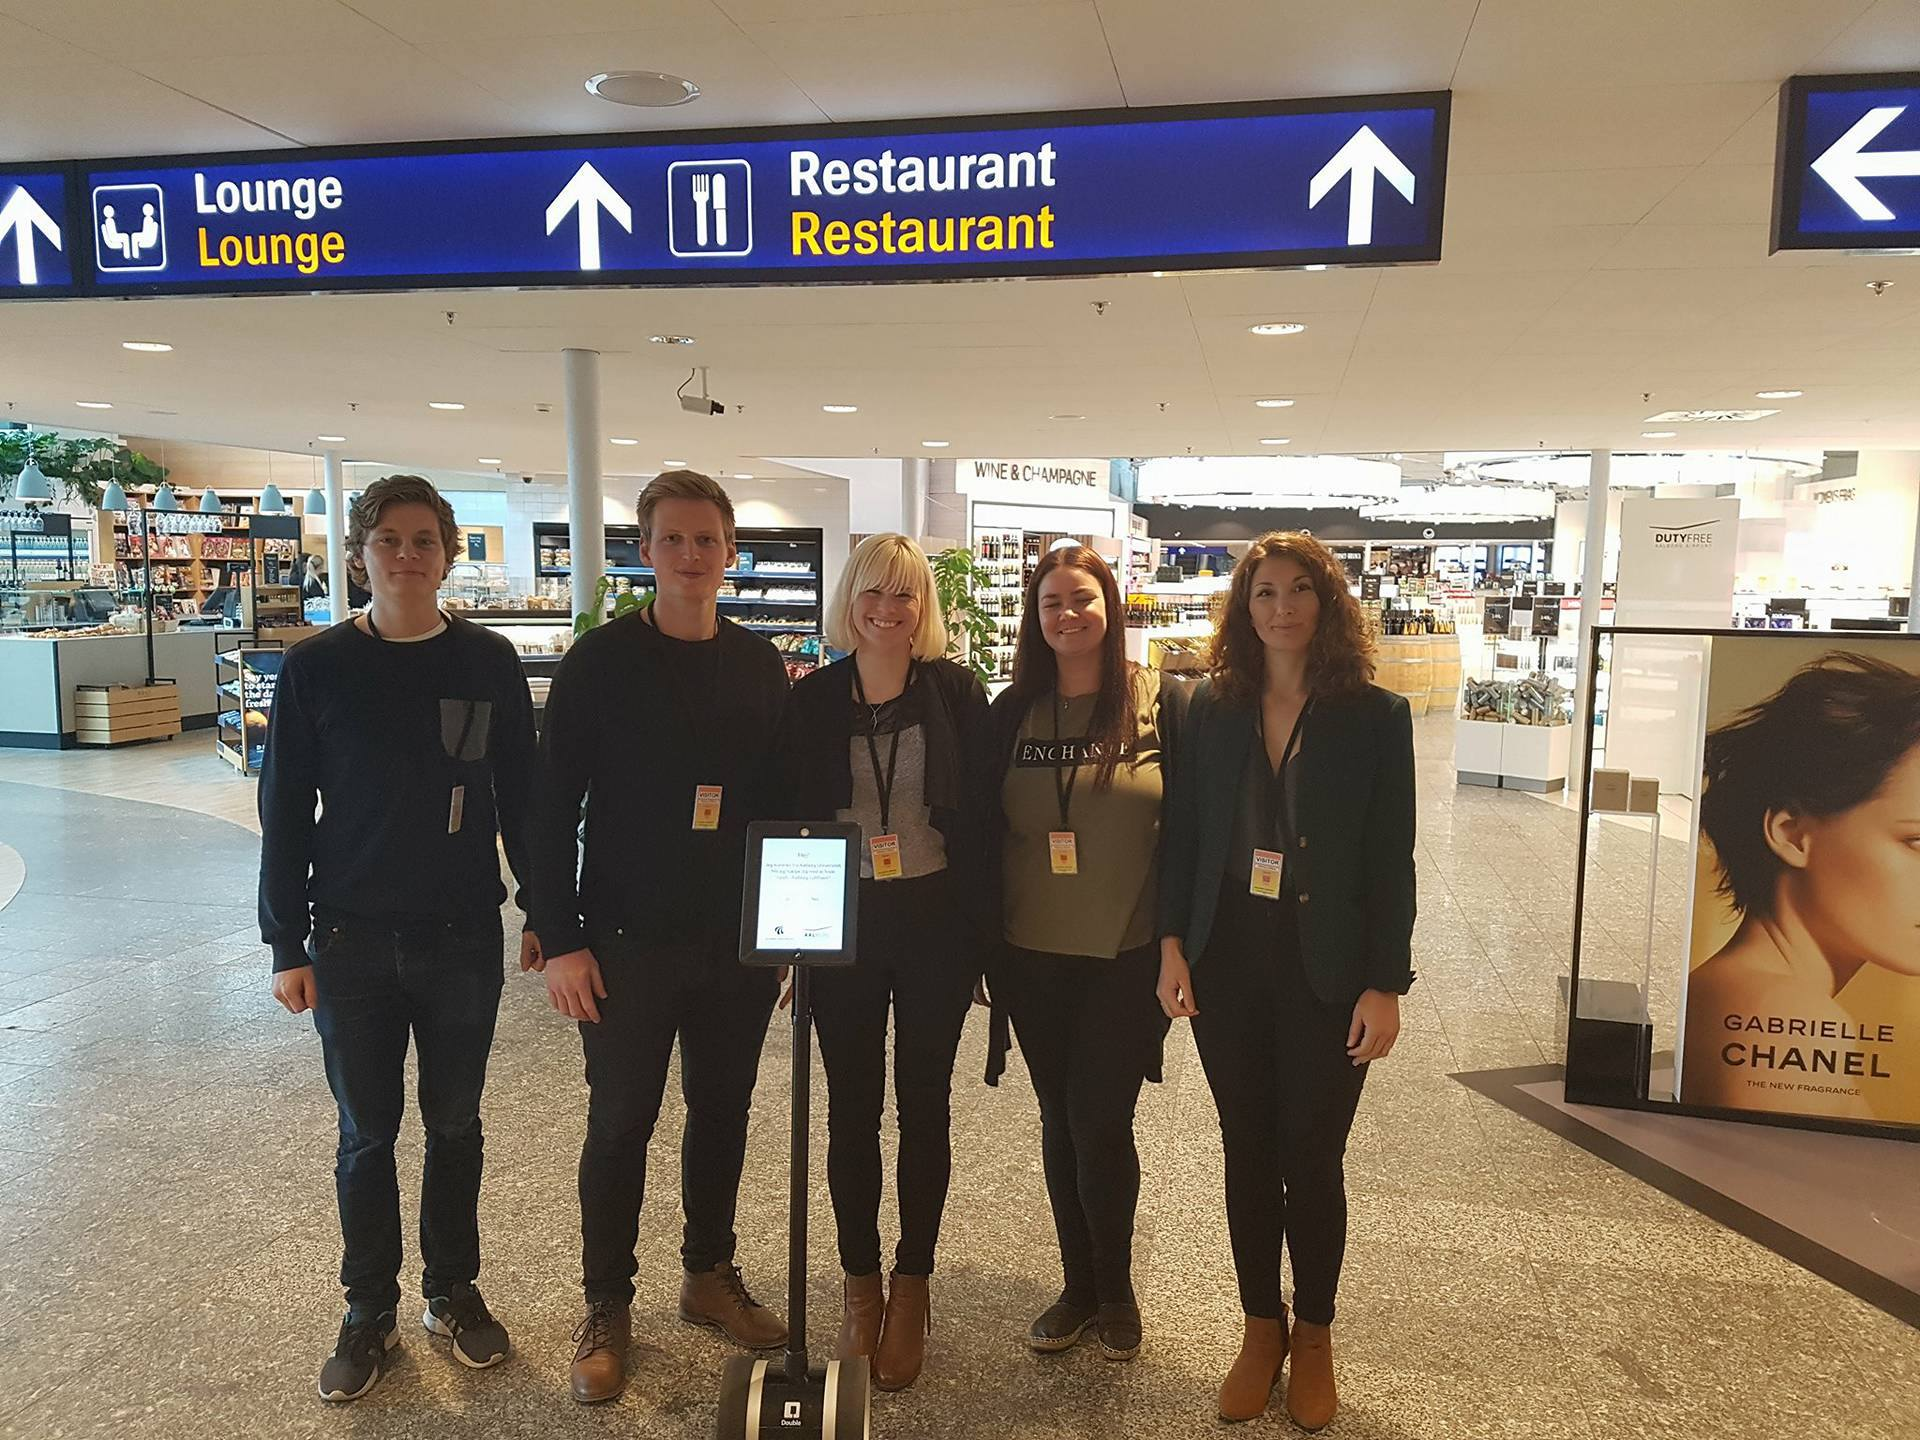
\includegraphics[width = 0.75\textwidth]{Figure/FrontPagePic} 
\label{fig:CategorizationOfRobots}
\end{figure}
\noindent 
%
\begin{center}
\large{\textbf{Gruppemedlemmer}:} \\
\groupmemberI \\\hspace*{1ex}
\groupmemberII \\\hspace*{1ex}
\groupmemberIII \\\hspace*{1ex}
\groupmemberIIII \\\hspace*{1ex}
\groupmemberIIIII \\\hspace*{1ex}
\end{center}

\printauthor% Print the author data as defined above
\restoregeometry %Forside
\cleardoublepage\tableofcontents* %Indholdsfortegnelse

\mainmatter	%Starter med at nummerere siderne
%
\newcommand{\Intorduktionpartname}{Introduktion}
\newcommand{\Introduktionparttext}{Ny
\newpage 
}
%
\part[\Intorduktionpartname]{\Intorduktionpartname
\label{\Intorduktionpartname}
\vspace{8mm}
	\begin{center}
		\begin{minipage}[l]{14cm}
			\textnormal{\normalsize\noindent\Introduktionparttext}
		\end{minipage}
	\end{center}
}
\chapter{Projekt retning}
\label{ProjektRetning}
%
Følgende kapitel er en redegørelse over projektets retning. Indholdet er blevet sendt til vejleder Dort Hammershøi, den 5. oktober 2017, samt Karl Damkjær Hansen, som står bag projektforslaget, den 10. oktober 2017. Da dette er første udkast omkring projekt retning, skal der tages forbehold for ændringer.
%
\section{Formål}
\label{ProjektRetningFormaal}
%
Projektets formål er at undersøge den subjektive oplevelse af en interaktion mellem mennesker og sociale robotter i forskellige kontekster, med henblik på implementering af primitiv social intelligens, som skal gøre robotten i stand til at interagere med mennesker på en social acceptabel måde.\blankline
%
Projektforslaget startede med et besøg i Karl Damkjær Hansens robotlaboratorium. Karl udvikler sociale robotter som kan køre hen til mennesker og indgå i forskellige interaktioner med dem. Karls primære arbejdsområde er det tekniske aspekt i at få robotterne til at køre som de skal. Han har indtil videre arbejdet med nogle forskellige modeller, blandt andet en robotstøvsuger og en segway lignende platform. For at give robotterne en mere menneskelig adfærd er der et ønske om at gøre dem mere dynamiske i deres bevægelser og ydermere gøre dem i stand til at bevæge sig i alle retninger. Begge dele gør dem i stand til at bevæge sig tilsvarende den måde mennesker underbevidst bevæger sig på, når de eksempelvis skifter vægten fra det ene ben til det andet eller gør en samtalekreds større, for at gøre plads til flere mennesker. 

Derfor arbejder Karl nu på at udvikle en robot som balancerer på en kugle og bruger inerti til at kunne bevæge sig i alle retninger. Kuglens store diameter gør at robotten kan køre ubesværet og naturligt på de fleste overflader og da den hele tiden står og holder balancen på kuglen, føles den også lidt mere levende at interagere med.
%
\section{Case: Lufthavn}
\label{CaseLufthavn}
%
Karl har indtil videre arbejdet med en case, hvor robotterne skulle indgå i et genoptræningsprogram og hjælpe folk til at lave øvelserne rigtigt. En anden case han har arbejdet med er Hotel Scandic i Aalborg, som ønskede at have en robot som kan byde gæster velkommen og checke dem ind, men også tage imod bestillinger fra hotelbarens gæster. På nuværende tidspunkt handler projektet for Karl om at få robotterne til at bevæge sig på en hensigtsmæssig måde, så de kan indgå i en social interaktion. Fra februar starter han et nyt overbyggende projekt i samarbejde med Combine og Københavns lufthavn. Formålet med dette projekt er at få udviklet robotterne, så det er nemt for udviklere eller designere at programmere robotterne til den specifikke kontekst den skal indgå i. Idéen er efterfølgende, at digitale bureauer, eksempelvis Combine, kan tilbyde deres kunder en robot, på lige fod med at de sælger applikationer og hjemmesider. Som en case for dette projekt, bruger de Københavns lufthavn, som allerede nu er meget interesserede i at få en robot ud og servicere deres kunder.\blankline
%
I lufthavne kan der hurtigt opstå en kaotisk stemning, når folk løber rundt på gangene for at nå deres fly. Et af de største problemer er ofte, at folk ikke er klar over hvor god tid de egentlig har og hvor langt de skal gå, og derfor skynder sig ned mod gaten. Når de når derned, er de langt væk fra salgsområderne, som typisk ligger centralt i lufthavne, hvilket resulterer i at de enten ikke køber noget, eller at de går frem og tilbage endnu en gang. Det påvirker blandt andet folks oplevelse af lufthavnen og rejsen, men også butikkernes omsætning. Københavns lufthavn vil gerne forsøge at holde folk i de centrale dele af lufthavnen længst muligt og dermed minimere trafikken på gangarealerne ud mod de forskellige gates. Det er her robotterne kommer ind i billedet, da disse kan fungere som serviceassistenter. Det forestilles, at robotterne kan køre rundt og fortælle folk, hvor længe der er til deres gate lukker, hvor langt der er derhen samt hvor de kan finde eller aflevere bagage. Ydermere forestilles det, at robotterne kan vise vej til gaten og eventuelt skabe mersalg i de centrale områder.
%
\section{Vores rolle}
\label{VoresRolle}
%
Ved møde med Karl blev det gjort klart, at der stadig er nogle udfordringer i forbindelse med den subjektive oplevelse af interaktionen med sociale robotter, før robotterne er klar til at komme ud og interagere med rigtige brugere. 

Det overordnede formål er at undersøge, hvordan robotterne skal indgå i en social kontekst og interagere med mennesker, hvortil følgende konkrete eksempler på problemer kan opstilles:\blankline
\begin{itemize}
  \item Hvordan skal robotten bevæge sig, sådan at dem vi vil interagere med føler, at den henvender sig til dem, uden at dem vi ikke vil interagere med føler at den også henvender sig til dem?
  \item Hvordan skal robotten forholde sig under en interaktion? Eksempelvis vippe, flytte sig fra side til side, dreje sig mod den der snakker, være dynamisk, stå stille osv.
  \item Hvordan skal robotten forholde sig, når nogen prøver at interagere med den fysisk? Eksempelvis når man skal trykke på touchskærmen.
  \item Hvordan skal robotten ændre adfærd, når der kommer nye mennesker ind i billedet?
  \item Hvordan kan folk ændre eksempelvis afstanden til robotten, hvis de føler at den er for nærgående eller for langt væk?
  \item Hvordan kan udseendet og interfacet på skærmen påvirke folks oplevelse?\blankline
\end{itemize}
\noindent
%
Ud fra ovenstående spørgsmål er det tydeligt, at der fra Karls side er meget fokus på at besvare spørgsmål i forbindelse med robottens overordnede sociale adfærd, som ikke er rettet mod en specifik case. Der ønskes at lave en generel løsning, som gør robotten i stand til at gebærde sig i mange forskellige situationer. Denne løsning omtales som robottens sociale intelligens.\blankline 
%
Der blev overvejet hvilke aspekter, der er vigtige i forbindelse med sociale robotters adfærd i de tre kontekster, som Karl arbejder eller har arbejdet med, Københavns lufthavn, Hotel Scandic Aalborg og et genoptræningscenter. Her blev der hurtigt enighed om, at robotten sandsynligvis ikke skal interagere med mennesker på samme måde i alle kontekster. Man kunne eksempelvis forestille sig, at folk i genoptræning, som inviterer robotten ind i deres hjem, vil have en anden oplevelse af robotten end folk i en lufthavn. Robotten bør i stedet tilpasses afhængigt af hvem den skal interagere med, hvad dens formål med interaktionen er og i hvilken kontekst interaktionen foregår.

For at gøre dette, kan der med fordel udvikles en metode eller en skala, som designere og udviklere i fremtiden vil kunne bruge til at evaluere den subjektive oplevelse i den specifikke kontekst, hvor robotten skal indgå. Ved evaluering af oplevelsen kan optimale bevægelsesmønstre findes, så de kan programmeres ind i robottens adfærd. Dette stemmer godt overens med Karls kommende projekt, som handler om at gøre robotter mere tilgængelige for almene virksomheder, ved at gøre det muligt for dem selv at programmere og tilpasse robotterne.

De udviklere og designere, som Karl har været i kontakt med, giver dog udtryk for at de ikke er interesserede i at involvere sig i, hvordan robotten bevæger sig. De vil foretrække at robotten har nogle foruddefinerede indstillinger for den grundlæggende måde robotten bevæger sig på, der gør at de kun skal tage stilling til hvad robotten skal gøre og ikke hvordan den skal gøre det. På den måde er det nemt og hurtigt for dem at programmere robotten til specifikke formål.

For at robotterne kan nå et niveau, hvor virksomhederne ønsker at de skal interagere med deres kunder, er det dog vigtigt at brugeroplevelsen optimeres til den givne kontekst, selvom det tager ekstra tid. Man kan derfor ikke altid bare bruge en generel model, som designeren eller udvikleren ellers ønsker. Samtidig er det dog værd at overveje, at hvis det er for omstændigt og dyrt at implementere robotterne, vil de digitale bureauer eller deres kunder sandsynligvis slet ikke købe dem. Det er derfor nødvendigt at finde et kompromis, som sikrer både en nem implementering og en skræddersyet brugeroplevelse, for at tilfredsstille alle interessenterne. 

\section{Potentielt løsningsforslag}
\label{PotentieltLoesningsforslag}
%
For at kunne udvikle denne primitive sociale intelligens i robotten, er det nødvendigt at forstå hvilke parametre brugeren mener er vigtige i en social robots adfærd. Ved at kigge på kontekster som eksempelvis lufthavne eller supermarkeder, hvor der er en meget bred målgruppe, kan det være muligt at udpege hvilke faktorer, der generelt er vigtige for robottens adfærd i disse situationer. På den måde behøves der ikke nødvendigvis laves dybdegående brugerundersøgelser og modificeringer hver gang robotten skal bruges i en ny kontekst, men der kan derimod generaliseres fra andre kontekster med samme karakteristika.

Når robotten skal bruges i kontekster med en mere snæver målgruppe og med et mere specialiseret formål, kan det derimod være nødvendigt at lave brugerundersøgelser for den enkelte situation og modificere robottens adfærd herefter. 

I dette projekt tages der udgangspunkt i casen om Københavns lufthavn, hvor det undersøges, hvordan folk oplever interaktionen med robotten. Potentielle brugere vil blive interviewet, med henblik på at finde generelle tendenser i deres subjektive oplevelser med den sociale robot. Disse tendenser bruges til at udvikle en eller flere skalaer til evaluering af brugeroplevelsen. Skalaerne kan herefter verificeres med andre potentielle brugere. Hvis de vigtige parametre kan generaliseres til også at gælde andre lignende situationer, som eksempelvis et shoppingcenter, sygehus eller supermarked, vil de udviklede skalaer sandsynligvis kunne bruges til at teste robottens adfærd i nævnte, lignende situationer.

Der startes med et lille studie, der forsøger at afdække hvordan folk snakker om oplevelsen med robotten og især hvilke ord folk bruger til at beskrive deres oplevelse. Det gøres for at være sikker på, at skalaerne udvikles ud fra de reelle brugeres egne forståelser. Derefter vil et forsøgsdesign blive opstillet som tester præcist de parametre, som vi har fundet ud af er vigtige for robottens sociale adfærd.

\chapter{Sociale robotter}
\label{SocialRobot}
%
I det følgende kapitel vil der først blive specificeret hvad der karakteriserer en social robot og herunder belyses det hvilke eksisterende sociale robotter, der allerede er på markedet. Dernæst vil projektsamarbejdet blive yderlige specificeret. Efterfølgende fokuseres der på teknologier i lufthavne, hvorefter interaktion og udfordringer ved sociale robotter belyses. Afslutningsvist ledes der over i en problemformulering, som danner grundlag for det fremadrettede projektarbejde.
%
\section{Karakterisering af social robot}
\label{KarakteriseringAfSocialRobot}
%
Sociale robotter adskiller sig fra industrielle robotter, da det overordenede formål er, at de skal tage sig af mennesker, \parencite[s. 13]{PDF:RobotShiftFromIPtoSR}. Sociale robotter skal særligt tage sig af de svage i samfundet; ældre, handicappede, syge og børn, \parencite[s. 14]{PDF:RobotShiftFromIPtoSR}. Formålet med industrielle robotter er, at de kan udfører farligt og gentagende arbejde, hvorfor de potentielt kan rede menneskeliv, \parencite[ss. 12-13]{PDF:RobotShiftFromIPtoSR}. På \autoref{fig:CategorizationOfRobots} illustreres en kategorisering af robotter, hvor det blandt andet fremgår at industrielle robotter og sociale robotter ikke tilhører den samme robottype.    
%
\begin{figure}[H]
\centering
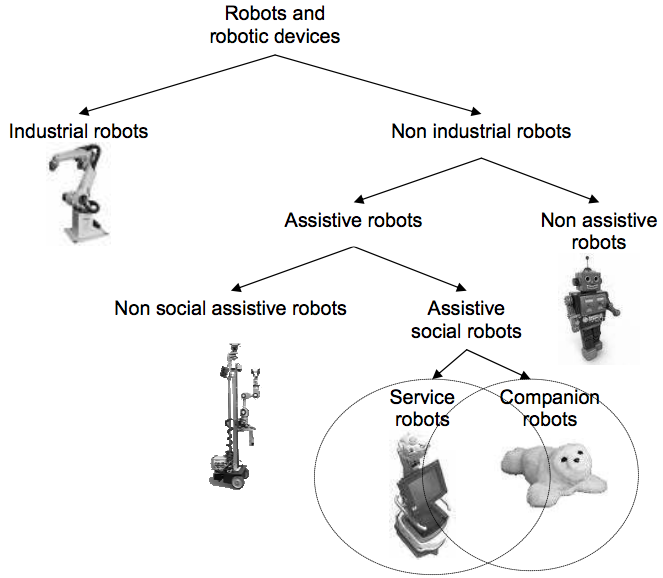
\includegraphics[width = 0.75\textwidth]{Figure/CategorizationOfRobots} 
\caption{Kategorisering af robotter fremsat af \textcite[s. 13]{PDF:AssesingAcceptance}.}
\label{fig:CategorizationOfRobots}
\end{figure}
\noindent 
%
Da projektet fokuserer på sociale robotter, \textit{Assistive social robots}, som skal indgå i en kontekst blandt mennesker, afgrænses der fra industrielle robotter, \textit{Non assistive robots} samt \textit{Non social assistive robots}. Sidstnævnte robottype er en form for fysisk teknologisk hjælpemiddel, der kan anvendes til rehabilitering, det kan eksempelvis være proteser eller intelligente kørestole, \parencite[s. 12]{PDF:AssesingAcceptance}.    

Ifølge \textcite[s. 1]{PDF:SharingALifeHarvey} kan sociale robotter karakteriseres ved, at de har forståelse og evne til at kommunikere på en menneskeagtig måde, hvilket gør det muligt for deres brugere at forstå dem. I tillæg argumenterer \textcite[s. 168]{PDF:TowardSociableRobots} for, at når mennesker enten observerer eller interagerer med en autonom robot tildeles den en social model. For at en autonom robot kan kategoriseres som en social robot skal den, ifølge \textcite[s. 168]{PDF:TowardSociableRobots}, percipere omgivelserne, tage selvstændige beslutninger og udføre koordinerede handlinger for at løse deres opgave. Da sociale robotter designes til at interagere med mennesker, via simpel kommunikation, vil det øge brugerens accept af robotten \parencite[s. 1476]{PDF:ExploringInfluencingVariable}. Ydermere forudser \textcite[s. 1476]{PDF:ExploringInfluencingVariable}, at sociale robotter i højere grad vil blive en del af vores hverdagsliv, og det er derfor nødvendigt at undersøge, hvordan mennesket perciperer sociale robotter og hvorfor de enten accepterer eller afviser dem \parencite[s. 1]{PDF:SharingALifeHarvey}.  




\subsection{Eksisterende sociale robotter}
\label{EksisterendeSocialeRobotter}
%
LAV FIGUR MED DE FORSKELLIGE ROBOTTER\blankline
%
Der findes et stort udvalg af sociale robotter når det kommer til børnelegetøj, blandt disse er den nok bedst kendte Sony's \textit{AIBO}, som er en robot hund, \parencite{WEB:AIBO}. AIBO er designet til at udvikle sin personlighed fra hvalp til voksen, afhængigt af interaktionen med dens ejer og omgivelser, \parencite{WEB:AIBO}. Selvom AIBO ikke er en virkelig hund, afspejler den hundes naturlige bevægelsesmønstre og behov, \parencite[ss. 191-198]{PDF:AnEthologicalEmotional}. Det resulterer i at ejeren tildeler AIBO hunde-agtige egenskaber, hvorved den behandles som en social ledsager med mentalkapacitet, \parencite[s. 2]{PDF:SharingALifeHarvey}. Dette kommer blandt andet til udtryk ved en analyse af kommentarer i et forum, hvor 47 \% tildeler AIBO en biologisk essens, 42 \% vurderer at AIBO har forsætlig adfærd, 38 \% vurderer at AIBO har følelser og 39 \% vurderer at AIBO kan opdrages, udvikles og modnes, \parencite[s. 26]{PDF:InTheCompanyofRobots}. En anden social robot, som ligeledes anvendes blandt børn er \textit{NAO}, designet af \textcite{WEB:NAO}. \textit{NAO} er en robot, der kan bruges til undervisning.  

I forbindelse med autistiske børn tyder det ligeledes på, at sociale robotter kan anvendes som en del af barnets terapi, \parencite[s. 180]{PDF:GamesChrildrenAutism}. Ifølge \textcite[s. 185]{PDF:GamesChrildrenAutism} er en af fordelene ved at anvende en robot, \textit{Roberta}, at den er mindre kompleks end mennesker, hvilket gør det muligt for robotten at hjælpe barnet med at udvikle sociale kompetencer. 

Ydermere kan sociale robotter ligeledes indgå som en form for terapi for ældre, som eksempelvis lider at demens eller oplever ensomhed, \parencite[s. 110]{PDF:TheMobilePhoneAnEmontionalisedSR}. \textit{PARO}, som er en robot sæl, anvendes blandt andet i disse situationer. Ifølge \textcite{WEB:PARO}, reducerer \textit{PARO} patientens stress, gør dem mere afslappet og motiveret og forbedre socialeegenskaber. Udover \textit{PARO}, findes \textit{ROMEO}, som er designet til at hjælpe ældre og andre der har mistet en del af deres mobilitet, \parencite{WEB:ROMEO}. I forhold de før nævnte robotter er \textit{ROMEO} forholdvis stor; 140cm høj. Ved at introducerer sociale robotter, designet til at hjælpe ældre, kan det være med til at sænke belastningen på sundhedsystemet i takt med at den ældre har mulighed for et længere uafhængigt og sundere liv i sit eget hjem, \parencite[s. 1]{PDF:SharingALifeHarvey}.\blankline
%
\textit{Double} tillader at medarbejdere kan arbejde hvor som helst og gennem robotten være til stede på arbejdspladsen samtidig, \parencite{WEB:Double}. En lignende form for telekommunikation opleves med \textit{HUGVIE}, som er en menneskeformet pude med hovede, arme, krop og ben, \parencite[s. 78]{PDF:MinimizingTheHuman}. I \textit{HUGVIE}s hovede er det muligt at lægge en mobiltelefon i en lomme og dermed fører en samtale, eksempelvis med ens partner, samtidig med at brugeren krammer \textit{HUGVIE} og mærker dens hjertebanken, som afspejler den transmiterede lyd.

Derudover anvendes sociale robotter som turguider og receptionister på museer, \parencite[s. 22]{PDF:CloseButNotStuck}.
\section{Projektsamarbejde}
\label{ProjektSamarbejde}
%
Projektet dækker over et samarbejde mellem projektgruppen, inklusiv vejleder, og Karl Damkjær Hansens, som er ansat ved Aalborg Universitet. Karls arbejde involverer udviklingen af sociale robotter, som skal indgå i en menneske-robot interaktion, \textit{Human-Robot Interaction}, HRI. Dertil fokuseres der på, hvordan den sociale robot skal henvende sig til interaktionspartneren(e), hvor Karl's primære arbejdsområde dækker det tekniske aspekt. Da sociale robotter skal kunne indgå i HRI er det en fordel at robotten afspejler menneskelig adfærd, eksempelvis i forhold til bevægelsesmønstre, hvor målet dels er at få robotten til at udføre dynamiske bevægelser og dels tillade robotten friheden til at bevæge sig 360$^{\circ}$. Ved at opfylde de to mål bør det være muligt at få robotten til at gengive menneskelige bevægelser såsom vægtfordeling under en stående samtale samt øge samtalekredsen for at inkludere én eller flere samtalepartnere.

For at muliggøre dette arbejder Karl med at udvikle en robot, som balancerer på en kugle (FIND UD AF HVOR STOR KUGLEN ER!), hvilket tillader 360$^{\circ}$ bevægelse, og i tillæg benyttes inerti til at gengive menneskelige bevægelser. Ved at balancere robotten på en kugle gør det, det muligt ikke blot at bevæge sig frem og tilbage men også sidelæns, hvilket eksempelvis ikke er tilfældet ved \textit{Double}, \parencite{WEB:Double}, som balancerer på en cylinder. Fælles for Karl's robot og \textit{Double} er, at de begge benytter sig inerti, for at gengive menneskelige bevægelser, såsom vægtfordeling. Kuglens store diameter tillader robotten at køre ubesværet og naturligt på de fleste overflader og i tilfæde hvor robotten skal køre over et dørtrin, så vil det fremstå flydende og ikke skramlende, som er tilfældet ved en mindre kugle diameter. Robotten er illustreret på XX INDSÆT BILLEDE.\blankline 
%
%INDSÆT BILLEDE AF ROBOTTEN måske ved siden af Double
%   
Formålet med robotten er, at den skal indgå i Københavns Lufthavn, hvor den eksempelvis skal hjælpe de rejsende med at finde frem til deres gate i tide. At robotten skal indgå i Københavns Lufthavn udspringer fra samarbejdet mellem Karl, Combine og Københavns Lufthavn. De udviklere og designere, som Karl har været i kontakt med, giver udtryk for ikke at være interesserede i, hvordan robotten bevæger sig. De foretrækker at robotten har nogle foruddefinerede indstillinger for den grundlæggende måde hvorpå robotten bevæger sig, hvilket skal stemme overens med, hvad der forventes af en social robot. Derfor handler projektet for Karl om, at få robotten til at bevæge sig på en hensigtmæssig måde, så det er muligt for den at indgå i HRI. Det er med udgangpunkt i dette, projektsamarbejdet med Karl udspringer. 

Det overordnede formål med dette projekt er derfor, at undersøge dels hvordan robotten skal bevæge sig for at indgå i den sociale kontekst; Københavns Lufthavn, og dels hvordan den rejsendes subjektive oplevelse af interaktion er.\blankline
%  
For at udvikle den sociale intelligens i robotten, er det nødvendigt at undersøge hvilke parametre, der har indflydelse på den subjektive oplevelse af HRI. I følgende afsnit undersøges eksisterende sociale robotter, der allerede er på markedet, interaktion med sociale robotter, herunder hvilke parametre der har indflydelse på denne og efterfølgende undersøges udfordringer ved sociale robotter. SKRIV IND NÅR DET ER BESLUTTET HVOR DET OM LUFTHAVNEN SKAL VÆRE HENNE.   


\section{Lufthavne}
\label{Lufthavne}
%
Skriv lidt om hvad de har af teknologier, hvordan forskellige nationaliteter vurderer oplevelsen, hvordan kan det gøres bedre mm. 
\section{Interaktion med sociale robotter}
\label{InteraktionSocialeRobotter}
%
Inden der dykkes ned i hvilke parametre, der har indflydelse på hvordan interaktionen med sociale robotter perciperes og accepteres, vil nogle mere generelle tendenser blive diskuteret. Det dækker blandt andet over køns-, alders- samt kulturelleforskelle i henhold til synet på sociale robotter. Dernæst gives der nogle eksempler på, hvordan relaterede studier har målt brugerens perception og accept af sociale robotter.
%
\subsection{Generelle tendenser}
\label{InteraktionSocialeRobotterGenerelleTendenser}
%
I den vestlige verden er vi i langt mindre grad villige til at acceptere sociale robotter end hvad der eksempelvis er tilfældet i Japan, \parencite[s. 28]{PDF:InTheCompanyofRobots}. Det skyldes, ifølge \textcite[s. 28]{PDF:InTheCompanyofRobots}, at der er en indgroede frygt for maskiner og følelsen af manglende kontrol, hvilket ikke er tilfældet i den Japanske kultur, som åndeliggøre robotter. At mennesker i den vestlige verden frygter robotter kan, blandt andet, retfærdiggøres med at i 2012 angav 87 \% af borgerne i Europa, at de aldrig har været i kontakt med en robot, hverken i hjemmet eller på ens arbejdsplads, \parencite[s. 40]{PDF:PerceptionAcceptance}. I en undersøgelse, beskrevet af \textcite[s. 41]{PDF:PerceptionAcceptance}, fremgår det at synet på robotter ikke har ændret sig de sidste 35 år. Når robotterne, ved brug af tegninger, visualiseres så minder de i høj grad om robottypen: \textit{Non assistive robots}, illustreret på \autoref{fig:CategorizationOfRobots}. Endvidere tyder det på, at Europærer frygter, at de vil miste deres job til robotten og at robotten er til for at erstatte mennesket, \parencite[s. 22]{PDF:RobotShiftFromIPtoSR}.   

Derudover er der en tendens til, at mænd i højere grad perciperer robotten som menneskeagtig sammenlignet med kvinder, som i langt højere grad perciperer robotten som en maskine, \parencite[s. 28]{PDF:InTheCompanyofRobots}. Ifølge \textcite[s. 1479]{PDF:ExploringInfluencingVariable}, perciperer mænd robotter som værende mere brugbare, de har større intention om at bruge dem og de er mere villige til at acceptere robotter end kvinder er.  

Ydermere argumenterer \textcite[s. 2]{PDF:SharingALifeHarvey} for, at den ældre population i højere grad accepterer sociale robotter, sammenlignet med den yngre population. Det antages, at en af årsagerne til det formentlig skyldes, at der anvendes sociale robotter i ældreplejen eksempelvis til mindske følelsen af ensomhed, \fullref{EksisterendeSocialeRobotter}. I mere praktiske situation, som eksempelvis rengøring, tøjvask og lignende, foretrækker ældre robotter fremfor mennesker, hvorimod hvis opgaverne er omsorgsrelateret foretrækkes mennesker, \parencite[s. 22]{PDF:RobotShiftFromIPtoSR}.

\subsection{Parametre, der har indflydelse på accept og interaktion med sociale robotter}
\label{InteraktionSocialeRobotterParametre}
%
\textcite[s. 1477]{PDF:SharingALifeHarvey} opstiller tre forskellige problemstillinger, der bør overvejes når brugerens accept af en social robot undersøges. I de følgende afsnit undersøges hvilke parametre, der har indflydelse på brugerens accept i forhold til de tre problemstillinger:\blankline 
%
\begin{quotation}
\textit{
  \begin{enumerate}
  \item the likely positive or negative consequences of the behavior
  \item the approval or disapproval of the behavior by respected individuals or groups, and
  \item the factors that may facilitate or impede performance of the behavior.
\end{enumerate}}
\textcite[s. 1477]{PDF:SharingALifeHarvey}\blankline
\end{quotation}
\noindent
%
Overvejelserne afspejler henholdvist brugerens evaluering af robotten, hvilke sociale normative overbevisninger, der tilskrives robotten ved brug samt hvilke kontekstuelle faktorer, der spiller ind ved brug, \parencite[s. 1477]{PDF:SharingALifeHarvey}. Baseret på \textcite[ss. 1477-1478]{PDF:SharingALifeHarvey} tyder det på, at der er to overordnede kategorier af parametre, som har indflydelse på den første problemstilling: Utilitaristiske og hedoniske parametre. Førstnævnte dækker over det praktiske og anvendelige aspekt ved at interagere med en social robot, hvor sidstnævnte relateres til brugerens oplevelse af at anvende den sociale robot, \parencite[s. 1476]{PDF:SharingALifeHarvey}.

I følgende to afsnit vil de utilitaristiske og hedoniske parametre undersøges nærmere, hvorefter de sociale normative overbevisninger og efterfølgende hvilke parametre, der har indflydelse på præstationsevnen, undersøges.
%   

\subsubsection*{Utilitaristiske parametre}
\label{InteraktionSocialeRobotterParametreUtilitarian}
%
Som nævnt dækker utilitaristiske parametre over det praktiske og anvendelige aspekt ved at interagere med en social robot. Derudover har disse parametre ligeledes indflydelse på den specifikke adfærd. I følgende afsnit belyses hvilke parametre, der har indflydelse på det praktiske såvel som det anvendelige aspekt. Der tages primært udgangspunkt i \textcite[s. 1477]{PDF:SharingALifeHarvey}.
%
\begin{figure}[H]
\centering
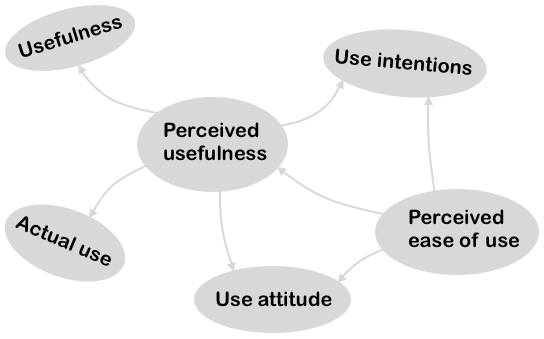
\includegraphics[width = 0.75\textwidth]{Figure/UtilitarianParameters} 
\caption{Sammenhængen mellem de seks forskellige parametre, der har indflydelse på det praktiske og anvendelige aspekt. Pilene indikerer hvilken retning indflydelsen er mellem to parametre.}
\label{fig:UtilitarianParameters}
\end{figure}
\noindent 
%
Baseret på \textcite[s. 1477]{PDF:SharingALifeHarvey} defineres \textit{usefulness} som værende brugerens overbevisning om, at robotten vil forbedre de daglige aktiviteter. Ifølge \textcite[s. 11]{PDF:SharingALifeHarvey} tyder det på, at \textit{usefulness} er en vigtig parametre, der kan bidrage til langtidssigtet forhold mellem bruger og robot. \textit{Ease of use} defineres som værende brugerens overbevisning om, at det nemt at anvende robotten. Derudover argumenterer \textcite[s. 1477]{PDF:SharingALifeHarvey} for, at i situationer hvor robotten skal indgå i en social interaktion med mennesker, er det nødvendigt at robotten gengiver menneskeagtige træk, for at brugeren føler sig komfortabel nok til at indgå i interaktionen. Robottens evne til at tilpasse sig den sociale kontekst afhængigt af brugeres behov, defineres som \textit{perceived adaptability}. Ifølge \textcite[s. 1477]{PDF:SharingALifeHarvey}, har \textit{perceived adaptability} indflydelse på \textit{perceived usefulness}, \textit{use attitude}, \textit{use intentions}, som er repræsenteret på \autoref{fig:UtilitarianParameters}. Derudover har \textit{perceived adaptability} indflydelse på \textit{enjoyment}. Ydermere tyder det på at \textit{intelligence}, har en effekt på hvor realistiske robotten perciperes, \parencite[s. 1477]{PDF:ExploringInfluencingVariable}.   
%
\subsubsection*{Hedoniske parametre}
\label{InteraktionSocialeRobotterParametreHedonic}
%
Som nævnt dækker hedoniske parametre over brugerens oplevelse af at anvende den sociale robot. Derudover har disse parametre ligeledes indflydelse på den specifikke adfærd. I følgende afsnit belyses hvilke parametre, der har indflydelse på det dette. Der tages primært udgangspunkt i \textcite[ss. 1477-1478]{PDF:SharingALifeHarvey}. På \autoref{fig:HedonicParameters} illustreres forskellige parametre, samt deres indbyrdes forhold.
%
\begin{figure}[H]
\centering
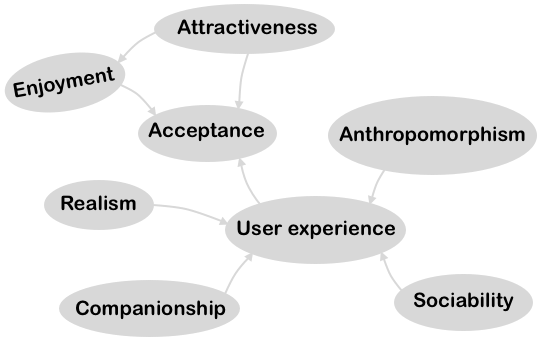
\includegraphics[width = 0.75\textwidth]{Figure/HedonicParameters} 
\caption{Sammenhængen mellem de otte forskellige parametre, der har indflydelse på brugerens oplevelse. Pilene indikerer hvilken retning indflydelsen er mellem to parametre.}
\label{fig:HedonicParameters}
\end{figure}
\noindent 
%
Baseret på \textcite[s. 1477]{PDF:ExploringInfluencingVariable} har både \textit{enjoyment}, der defineres som værende følelsen af fornøjelse eller glæde forbundet med brug, og \textit{attractiveness}, der defineres som værende den positive evaluering af robottens udseende, på flere af de parametre gengivet på \autoref{fig:UtilitarianParameters}. \textit{Enjoyment} har indflydelse på \textit{ease of use}, \textit{use attitude} samt \textit{use intentions}. Derimod har \textit{attractiveness} indflydelse på \textit{usefulness} og \textit{ease of use}. \blankline 
%
Antropomorfisering defineres som værende evnen til at tilskrive naturfænomener, guder, overnaturlige væsner og dyr menneskelige egenskaber, såsom følelser og motiver, \parencite{WEB:DefAntropomorisering}. Dog defineres antropomorfisering i HRI sammenhæng, som værende evnen til at tildele og beskrive objekter med menneskelige egenskaber, for at rationalisere objektets adfærd, \parencite[s. 1478]{PDF:ExploringInfluencingVariable}. Ifølge \textcite[s. 1478]{PDF:ExploringInfluencingVariable} har anthropomorfisme indflydelse på \textit{usefulness}, \textit{use attitude} samt \textit{use intention}, som er repræsenteret på \autoref{fig:UtilitarianParameters}. Derudover har \textit{anthropomorphism} ligeledes indflydelse på \textit{attitude toward robots}, \textit{social influence} samt \textit{companionship}. Ifølge \textcite[s. 19]{PDF:CloseButNotStuck} resulterer antropomorfisering i, at mennesket betragter en social robot som en social enhed, hvorfor robotten behandles som et menneske.

Der er forskellige årsager til at mennesker antropomorfiserer sociale robotter. Antropomorfisering kan forekomme i situationer hvor mennesket oplever en manglende kontrol og usikkerhed, hvor mennesket i højere grad har en tendens til at antropomorfisere sociale robotter, for at kunne forstå, kontrollere samt forudse robottens adfærd, \parencite[s. 1478]{PDF:ExploringInfluencingVariable}. Dette høre under \textit{effectance motivation}, der defineres som værende ønsket om effektivt at kunne interagere med ens omgivelser, \parencite[s. 62]{PDF:EffectsOfAnticipatedHRI}.

Derudover har mennesker med en teknologisk baggrund en tendens til at tildele robotten sin egen personlighed, hvilket ikke er tilfældet med mennesker uden teknologisk baggrund, \parencite[s. 19]{PDF:CloseButNotStuck}. I tillæg argumenterer \textcite[s. 2]{PDF:SharingALifeHarvey} for, at desto mere antropomorfisering brugeren oplever, desto bedre er evalueringen af robotten, desto mere fornøjet er de med interaktionen og desto større er chancen for at de oplever robotten som en ledsager.

Ifølge \textcite[s. 61]{PDF:EffectsOfAnticipatedHRI} har ensomme mennesker en stærk tendens til at antropomorfisere kæledyr og teknologiske objekter, såsom robotter. Det skyldes, at mennesket har et behov for både tilknytning og et tilhørsforhold. Dette hører under \textit{sociality motivation}, der defineres som værende ønsket og behovet for at skabe en social relation til andre, \parencite[s. 61]{PDF:EffectsOfAnticipatedHRI}. I det henseende vil en robot med et mere livagtigt udtryk perciperes som værende en venlig ledsager, \parencite[s. 1478]{PDF:ExploringInfluencingVariable}. Dette gengives som \textit{companionship}, der defineres som brugerens perciperede mulighed for at bygge et forhold til robotten. \textit{Companionship} er illustreret på \autoref{fig:HedonicParameters} og udover at have indflydelse på \textit{user experience}, har \textit{companionship} indflydelse på den vedvarende interaktion med robotten. \blankline
%
Baseret på \textcite[s. 1478]{PDF:ExploringInfluencingVariable} tyder det på, at \textit{realism} kan forbedre HRI og har dermed indflydelse på \textit{user experience}, \autoref{fig:HedonicParameters}. En robots \textit{realism} afspejler i hvilken grad brugeren tro på, at robotten reagerer og opfører sig realistisk. Desto mere realistisk robotten perciperes, desto mere intelligent perciperes den, \parencite[s. 1478]{PDF:ExploringInfluencingVariable}. 

\textit{Sociability} defineres som værende brugerens overbevisning om hvorvidt robotten besidder de sociale, emotionelle samt kognitive færdigheder, der er nødvendige for en succesfuld tilvænning af robotten, \parencite[s. 1478]{PDF:ExploringInfluencingVariable}. Denne parameter har, ifølge \textcite[s. 1478]{PDF:ExploringInfluencingVariable}, ligeledes indflydelse på \textit{use attitude} og \textit{usefulness}.\blankline
%
I henhold til teknologier i lufthavne argumenterer \textcite[s. 352]{PDF:TheImpactOfTraveler} for, hvorfor der bør tages højde for \textit{hedonic} parametre. En stor del af den teknologi, som kan findes i lufthavne bygger primært på \textit{utilitarian} parametre, hvilket formentlig har været årsagen til en dårlig brugeroplevelse. For at forbedre dårlige oplevelser, blandt andet ved lange ventetider ved sikkerhedskontrollen, har lufthavne forsøgt at foretage nogle tiltag, der skal gøre oplevelsen bedre, hvilket eksempelvis kommer til udtryk ved et øget brug af smartphone applikationer. Derudover understreger \textcite[s. 352]{PDF:TheImpactOfTraveler}, at det er nødvendigt at skabe fornøjelige lufthavns oplevelser. Fornøjelighed gengives på \autoref{fig:HedonicParameters}, som \textit{enjoyment}.
%

\subsubsection*{Sociale normer}
\label{InteraktionSocialeRobotterParametreSocialeNormer}
% 
I henhold til problemstilling 2: \textit{the approval or disapproval of the behavior by respected individuals or groups}, fremsat af \textcite[s. 1477]{PDF:SharingALifeHarvey}, vil følgende afsnit undersøge hvilke parametre, der har indflydelse på det.\blankline
%
De sociale normer dækker over de synspunkter mennesket har i relation til deres egen adfærd og dækker ydermere de synspunkter og regler, der er gældende for en gruppe for hvorvidt en bestemt adfærd er passende eller upassende, \parencite[s. 1478]{PDF:ExploringInfluencingVariable}. Ifølge \textcite[s. 1478]{PDF:ExploringInfluencingVariable} dækker de sociale normer over \textit{social influence} og \textit{image}. \textit{Social influence} er karakteriseret ved brugerens perception af hvad andre tænker omkring brugen af robotten. Denne parameter har indflydelse på \textit{usefulness}, \textit{ease of use}, \textit{use attitude}, \textit{use intention} samt \textit{actual use}, \parencite[s. 1478]{PDF:ExploringInfluencingVariable}, jævnfør \autoref{fig:UtilitarianParameters}. Det er særligt mennesker i ens tætte omgangskreds; familie, partner og venner, hvis mening har indflydelse på hvorvidt en bestemt teknologi vil blive brugt, i dette tilfælde en social robot, \parencite[s. 1478]{PDF:ExploringInfluencingVariable}. 

\textit{Image} karakteriseres ved brugerens overbevisning om at interaktionen med robotten kan lede til større anerkendelse og social status blandt ens omgangskreds, \parencite[s. 1478]{PDF:ExploringInfluencingVariable}. Derudover har \textit{image} indflydelse på \textit{perceived usefulness}, illustreret på \autoref{fig:UtilitarianParameters}.\blankline
%
I relation til sociale normer og tilnærmelsesvis \textit{social influence} undersøger \textcite{PDF:HowSocialDistanceShapesHRI}, hvilken indflydelse \textit{social distance} har på HRI. \textit{Social distance} referer til hvilken grad mennesker perciperer manglende intimitet grundet forskellige egenskaber såsom etnicitet, race, religion, beskæftligelse, \parencite[s. 784]{PDF:HowSocialDistanceShapesHRI}. \textit{Social distance} dækker over to forskellige parametre; \textit{social structural distance} og \textit{physical distance}.

\textit{Social structural distance} referer til mennesket perception af og adfærd rettet mod andre, som er afhænger af hvordan mennesket kategoriserer andre, særligt i forhold til deres kompetance og varme, \parencite[s. 784]{PDF:HowSocialDistanceShapesHRI}. Derudover kategoriseres mennesker afhængigt af deres indbyrdes forhold, er der forskel i status, foregår interaktionen som samarbejde eller som en konkurrence. \textit{Social structural distance} kan inddeles i yderligere to kategorier; \textit{power distance} og \textit{task distance}. Førstnævnte har stor indflydelse på den individuelle's adfærd og perception afhængigt af forholdet til interaktionspartneren, som afhænger af personligheder, roller og deres individuelle sociale klasse, \parencite[s. 784]{PDF:HowSocialDistanceShapesHRI}. \textit{Task distance} referer til at mennesker afhænger af hinanden for at opnå deres mål, det kan enten komme positivt til udtryk når mennesker samarbejder for opnår deres fælles mål, eller negativt når mennesker konkurrerer mod hinanden og når de forhindre hinanden i at opnå deres individuelle mål, \parencite[s. 784]{PDF:HowSocialDistanceShapesHRI}. 

\textit{Physical distance} kan også beskrives som \textit{proxemic distance} og referer til den fysiske adskillelse mellem mennesker, \parencite[s. 784]{PDF:HowSocialDistanceShapesHRI}. Der opstår både bedre kommunikation mellem mennesker og den individuelle vil være i stand til at løse egne opgave bedre, \parencite[s. 785]{PDF:HowSocialDistanceShapesHRI}.\blankline
%
\textcite[s. 794]{PDF:HowSocialDistanceShapesHRI} undersøger forholdet mellem \textit{power distance} og \textit{proxemic distance} i forhold til HRI. \textit{Power distance} udtrykkes ved at robotten enten agerer som \textit{supervisor} eller som \textit{subordinate}, hvor \textit{proxemic distance} udtrykkes ved at afstanden mellem robot og menneske er lille eller stor. Baseret på disse resultater tyder det på, at \textit{user experience} blev bedre når interaktionen foregik med en \textit{supervisor} robot tæt på og når interaktionen foregik med en \textit{subordinate} robot langt væk, \parencite[s. 785]{PDF:HowSocialDistanceShapesHRI}. Dog finder \textcite[s. 785]{PDF:HowSocialDistanceShapesHRI}, at præstationen i opgaven blev forværret desto tætter robotten var på testpersonen, uafhængigt af \textit{power distance}. 

Derudover finder \textcite[s. 785]{PDF:HowSocialDistanceShapesHRI}, at \textit{user experience} blev forbedret når robotten konkurrerede med testpersonen tæt på og når robotten samarbejde med testpersonen langt væk, hvilket var imod forventningen, \parencite[s. 785]{PDF:HowSocialDistanceShapesHRI}.   
%
\subsubsection*{Indflydelse på præstationsevnen}
\label{InteraktionSocialeRobotterParametrePraestation}
%
I henhold til problemstilling 3: \textit{the factors that may facilitate or impede performance of the behavior}, fremsat af \textcite[s. 1477]{PDF:SharingALifeHarvey}, vil følgende afsnit undersøge hvilke parametre, der har indflydelse på præstationsevnen.\blankline
%
\textit{Control beliefs} referer til brugerens overbevisning om hvilke ressourcer, muligheder og forhindringer, der er tilstede eller fraværende og som vil have en positiv eller negativ indflydelse på præstationsevnen, \parencite[s. 1478]{PDF:ExploringInfluencingVariable}. \textit{Control beliefs} kan inddeles i tre kategorier, som alle har indflydelse på \textit{user acceptance}: \textit{Perceived behavioral control}, \textit{anxiety} og \textit{experience}, begge rettet mod robotter, \parencite[s. 1478]{PDF:ExploringInfluencingVariable}. 

\textit{Perceived behavioral control} defineres som værende brugerens perciperede oplevelse af hvor let eller svært det var at interagere med robotten, \parencite[s. 1478]{PDF:ExploringInfluencingVariable}. \textit{Perceived behavioral control} har indflydelse på \textit{perceived ease of use}, \textit{use intentions} samt \textit{actual use}. \textit{Anxiety} rette mod robotter defineres som værende ængstelige eller andre negative emotioner forbundet med HRI og som forværres afhængigt at tidligere oplevelser, \parencite[s. 1478]{PDF:ExploringInfluencingVariable}. \textit{Anxiety} har en negativ effekt på \textit{perceived ease of use}, men \textit{anxiety} kan reduceres med \textit{enjoyment}, \parencite[s. 1478]{PDF:ExploringInfluencingVariable}. 

\textit{Experience} med robotter defineres som den opnåede oplevelse med robotter både direkte, i form af HRI, og indirekte via et medie, såsom nyhedsartikler og science-fiction film, \parencite[s. 1479]{PDF:ExploringInfluencingVariable}. Som nævnt i \fullref{InteraktionSocialeRobotterGenerelleTendenser}, har 87 \% af borgerne i Europa aldrig indgået i en interaktion med en robot, hvorfor det antages at den direkte oplevelse med robotter er begrænset, hvert fald i Europæiske lande.

Tidligere erfaring med robotter har, ifølge \textcite[s. 1479]{PDF:ExploringInfluencingVariable}, en positiv effekt på: \textit{Usefulness}, \textit{ease of use}, \textit{attitude towards robots}, \textit{use intention} samt \textit{actual use}. I henhold til tidligere erfaringer med robotter, undersøger \textcite{PDF:CloseButNotStuck} hvorvidt \textit{online community} og erfaring med \textit{avatars}, har en indflydelse på evnen til at antropomorfisere og acceptere robotter. \textit{Community} defineres som forholdet mellem individet og den sociale struktur de tilhører, \parencite[ss. 20-21]{PDF:CloseButNotStuck}. Det essentielle ved \textit{community} dækker over support, \textit{sociability}, information, dannelse af social identitet og tilhørsforhold, \parencite[s. 21]{PDF:CloseButNotStuck}. Det eneste der, adskiller \textit{community} fra et \textit{online community} er, at sidstnævnte foregår på virtuelt. \textcite[s. 25]{PDF:CloseButNotStuck} fandt de testpersoner, som enten var en del af \textit{online community} eller mere involveret med \textit{avatars}, i højere grad var i stand til at genkende menneskelige træk ved robotten, sammenlignet med testpersoner uden disse erfaringer. Ydermere fandt \textcite[s. 26]{PDF:CloseButNotStuck} at testpersoner, som enten var en del af \textit{online community} eller mere involveret med \textit{avatars}, begge var mere villige til at acceptere robotter, som en del af deres sociale og fysiske miljø.  
%

\subsection{Bevægelsesmønstre og udseende}
\label{InteraktionSocialeRobotterParametreBevaegelsesmoenstre}
%
Som nævnt i \fullref{InteraktionSocialeRobotterGenerelleTendenser} forekommer der store kulturelle forskelle i forhold til hvordan sociale robotter perciperes. Ikke nok med det, forekommer der ligeledes store kulturelle forskelle i hvordan robotter bør bevæge sig, blandt andet i forhold til hvor tæt de må komme på. Først vil afstanden mellem robot og menneske blive diskuteret, og derefter hvilken hastighed robotten bør bevæge sig med. 

\subsubsection*{Afstand mellem robot og menneske}
\label{InteraktionSocialeRobotterParametreBevaegelsesmoenstreAfstand}
%
Ifølge \textcite[s. 178]{PDF:HowMayIServeYou} er den intime grænse for hvor tæt et andet menneske, tætte venner og familie, må komme på en mellem 20 cm og 30 cm for syd europærer og japanere. Hvorimod denne grænse for amerikanere og nord europæer er 46 cm til 122 cm. Ydermere har mennesker, der er opvokset i et landdistrikt ligeledes behov for en øget intim grænse, modsat mennesker, der er opvokset i bymiljøer, \textcite[s. 178]{PDF:HowMayIServeYou}. Endvidere tyder det på, at kvinder normalvis er tættere på hinanden og vendt mere direkte ansigt-til-ansigt, sammenlignet med mænd, \parencite[s. 178]{PDF:HowMayIServeYou}. Det må derfor antages at kvinder, har en mindre intim grænse end mænd.

I undersøgelsen foretaget af \textcite{PDF:HowMayIServeYou}, undersøger de blandt andet hvor tæt en robot må komme før den overskrider den intime grænse, afhængigt af indgangsvinkel: Frontal, højre eller venstre. Robotten holdte en afstand svarende til 50 cm $\pm$ 10 cm. I den første undersøgelse foretaget af \textcite[s. 174]{PDF:HowMayIServeYou}, angav 76 \% testpersonerne at afstanden mellem dem og robotten var \textit{about right}, 19 \% angav at afstanden var for stor og 5 \% angav at robotten kom for tæt på. I den anden undersøgelse foretaget af \textcite[s. 175]{PDF:HowMayIServeYou}, angav 53 \% af testpersonerne, at når robotten nærmede sig frontalt, at den kom for tæt på, 27 \% angav at afstanden var \textit{about right} og 20 \% angav af afstanden var for stor. Da robotten nærmede sig fra venstre, angav 80 \% af testpersonerne at det var \textit{about right} og 20 \% angav at afstanden var for stor. Da robotten nærmede sig fra højre, angav 60 \% af testpersonerne at afstanden var \textit{about right} og 40 \% angav at afstanden var for stor. I alle tilfælde foregår interaktionen mellem robotten og et siddende menneske.

I henhold til hvilken retning robotten skal nærme sig testpersonerne med fremgår det, at 59 \% foretrækker at robotten nærmer sig fra højre, 28 \% foretrækker venstre og 13 \% foretrækker frontalt, \parencite[s. 175]{PDF:HowMayIServeYou}. Lignende tendens går igen ved hvor praktisk og komfortabelt testpersonerne vurder interaktionen, \parencite[ss. 175-176]{PDF:HowMayIServeYou}. Der skal dog tages højde for kønsforskelle, da en del af kvinderne faktisk foretrækker at robotten nærmer sig frontalt, hvilket formentlig hænger sammen med at kvinder i højere grad interagerer med hinanden ansigt-til-ansigt, sammenlignet med mænd, \parencite[s. 178]{PDF:HowMayIServeYou}. Dog argumenterer \textcite[s. 178]{PDF:HowMayIServeYou} for, at den frontale indgangsvinkel opleves som værende ukomfortabel, upraktisk, truende og konfronterende, hvorfor det bør undgåes. I det henseende kommenterer \textcite[s. 178]{PDF:HowMayIServeYou} at i situationer, hvor der er en 45$^{\circ}$s vinkel mellem to samtale partnere, vil følelser som aggression og konfrontation være reduceret. Derudover skal der tages højde for at 94 \% af testpersonerne er højrehåndede, hvilket formentlig er årsagen til at størstedelen af testpersonerne foretrækker at robotten nærmer sig fra højre, \parencite[s. 175]{PDF:HowMayIServeYou}.\blankline
%
En anden undersøgelse, der blandt andet fokuserer på afstanden mellem robot og menneske, er foretaget af \textcite{PDF:HumanRobotEmodiedInteraction}. Der differentieres mellem fire forskellige afstande, som er gældende for menneske-menneske interaktion. \textit{Intimate distance} denne afstand går direkte fra kroppen til omkring 45 cm fra kroppen, og generelt beregnet til direkte fysisk kontakt eller privat interaktion \parencite[s. 165]{PDF:HumanRobotEmodiedInteraction}. Dernæst er \textit{personal distance}, som går fra 45 cm til 1,2 m, denne afstand gør sig gældende for interaktion med familie og venner eller ved organiserede interaktion, som opstår når mennesker står i kø, \parencite[s. 165]{PDF:HumanRobotEmodiedInteraction}. Den tredje afstand er \textit{social distance}, som går fra 1,2 m til 3,5 m og som er beregnet til mere formelle og arbejdsrelateret interaktioner, interaktioner med bekendte. Ydermere fungerer \textit{social distance} også som en form for separering mellem mennesker på offentlige steder, eksempelvis på stranden, \parencite[s. 165]{PDF:HumanRobotEmodiedInteraction}. Den sidste afstand er \textit{public distance}, som starter fra 3,5 m og anvendes i situationer, hvor der er envejskommunikation, eksempelvis mellem publikum og den optrædende, \parencite[s. 165]{PDF:HumanRobotEmodiedInteraction}.

Baseret på \textcite[ss. 169-170]{PDF:HumanRobotEmodiedInteraction} anbefales det, at når en robot skal passere et mennesker bør robotten signalerer det med en afstand på 4 m til 6 m fra mennesket, formentlig er en afstand på 3,5 m også acceptabelt, da det overholder \textit{public distance}. Såfremt robotten i tide signalerer dels at den nærmer sig og dels dens intention, som er at passere mennesket, er det ikke et problem at passagen foregår indenfor \textit{personal distance} og endda kan en mindre afstand også accepteres, \parencite[s. 170]{PDF:HumanRobotEmodiedInteraction}. I tillæg kommenterer \textcite[s. 170]{PDF:HumanRobotEmodiedInteraction}, at afstanden mellem robot og menneske under passagen er mindre vigtig så længe robotten signalerer sin intention i tide, så mennesket ligeledes kan reagerer på interaktionen, eksemplvist ved at bevæge sig til siden.    

\subsubsection*{Robottens hastighed}
\label{InteraktionSocialeRobotterParametreBevaegelsesmoenstreHastighed}
%
Ifølge \textcite[s. 165]{PDF:HumanRobotEmodiedInteraction} er den normale ganghastighed for et menneske mellem 3,6 km/h og 7,2 km/h, hvorfor det må forventes at en social robot ikke bør overskride det interval ved HRI. I undersøgelsen foretaget af \textcite[s. 175]{PDF:HowMayIServeYou} varierede robottens hastighed sig mellem 0,9 km/h og 1,44 km/h, hvor 60 \% af testpersonerne angav at hastigheden var \textit{about right} og 40 \% angav at hastigheden var for langsom. Ifølge \textcite[s. 178]{PDF:HowMayIServeYou} bør en robot, efter en tilvænningsperiode eller efter behov, bevæge sig hurtigere end 1,44 km/h. 

I undersøgelsen foretaget af \textcite[s. 169]{PDF:HumanRobotEmodiedInteraction} svinger robottens gennemsnitlige hastighed mellem 0,9 km/h og 1,4 km/h. Årsagen til at robottens gennemsnitlige hastighed ikke er højere skyldes, at når robotten passerer et menneske sænkes hastigheden, \parencite[s. 169]{PDF:HumanRobotEmodiedInteraction}. Baseret på testpersonernes vurdering af robottens hastighed ville en højere hastighed være at foretrække, \parencite[s. 169]{PDF:HumanRobotEmodiedInteraction}. Ydermere tyder det på, at robottens lave hastighed blev perciperet som værende mindre sikker og tilmed irriterende, \parencite[s. 169]{PDF:HumanRobotEmodiedInteraction}, hvorfor der bør anvendes en højere hastighed. For at afgøre hvilken hastighed robotten bør bevæge sig med argumenterer \textcite[s. 167]{PDF:HumanRobotEmodiedInteraction} for, at robotten bør være i stand til at tilpasse sin hastighed afhængigt af menneskets hastighed, da dette vil medføre en mere dynamisk interaktion mellem robot og menneske. Ifølge \textcite[s. 1897]{PDF:NavigationForHRITasks} bør robotten sænke hastigheden når den nærmer sig en gruppe af mennesker, ligesom et menneske ville gøre det, hvis det nærmede sig en gruppe af mennesker.

\textcite[ss. 192-103]{PDF:PsychologicalEffects} undersøger tre forskellige hastigheder, fordelt på to måder robotten kan nærme sig et menneske på. Robotten kan enten nærme sig direkte eller indirekte, ved direkte er hastigheden enten 0,9144 km/h eller 3,6576 km/h og ved indirekte er hastigheden 1,8288 km/h, \parencite[ss. 192-103]{PDF:PsychologicalEffects}. En indirekte tilgang gengiver, at robotten først drejer mod venstre og derefter mod højre, hvilket giver en fornemmelse af at robotten bevæger sig en anelse til højre for mennesket, \parencite[s. 193]{PDF:PsychologicalEffects}. Med udgangspunkt i robottens hastighed fandt \textcite[s. 196]{PDF:PsychologicalEffects}, at den direkte hastighed på 3,6576 km/h var ubehagelig og at den indirekte hastighed på 1,8288 km/h var at foretrække, da den var mest behagelig. \blankline  
%
Baseret på de tre undersøgelser tyder det på, at hastigheder til og med 1,44 km/h i nogen grad kan accepteres, men det vil være, at foretrække hvis hastigheden var højere. Eftersom 1,44 km/h er langsommere end menneskets normale ganghastighed bør det være muligt, at øge robottens hastighed uden det påvirker interaktionen med mennesket negativt. Det lader rent faktisk til, at en øget hastighed potentielt kan forbedre interaktionen mellem robot og menneske, hvorfor der bør tages højde for dette. Dog tyder det på at robottens hastighed ikke må overstige mennesket normale ganghastighed.       
%

\subsubsection*{Robottens udseende}
\label{InteraktionSocialeRobotterParametreBevaegelsesmoenstreUdseende}
%




 In particular, it appears that for people to perceive a robot has having animate qualities, the robot does not have to have a humanoid appearance. Our observations suggest that the mere fact that the robot moves around in a non-predictable way may cause people to interpret it as acting intentionally, and as having a kind of personality. \textcite[s. 226]{PDF:SocailAndCollaborative}

 Apart from the explicitly humanoid characteristics that a robot may have, it seems clear that its size, shape, colour, and the character of its movements may be important. \textcite[s. 226]{PDF:SocailAndCollaborative}
 
 The results showed that the participants liked the happy robot more, but that they followed the robot’s instructions to a greater extent in the condition with the serious robot. It is con- ceivable that a robot’s personality would contribute to a user’s sense of trust in its instructions. \textcite[s. 226]{PDF:SocailAndCollaborative}
 
  Butler and Agah [5], the speed of a robot as well as its way of approaching a human affected people’s perceptions of it. Subjects were most comfortable with a slower robot, or a robot approaching indirectly rather than directly. Moreover, their reactions were affected by the robot’s exterior shape: the level of discomfort perceived during a fast approach increased if the robot had a tall and humanoid body rather than a short, neutral cylindrical shape. Smooth movements were preferred over jerky ones, and the distance to the robot was also a factor contributing to the subjects’ perception of comfort. Adding a tall, humanoid robot body attachment caused comfort levels to drop in all cases studied.\textcite[s. 226]{PDF:SocailAndCollaborative}
 
 
 
 
The height of the entire robot with the body attachment is about 67 inches. \textcite[s. 189]{PDF:PsychologicalEffects} 67 inches = 170,18 cm. Den har et hovede, krop og to arme (billedet på  \textcite[s. 192]{PDF:PsychologicalEffects}. 
 
Kom ind på uncanny valley






\chapter{Projektafgrænsning}
\label{Projektafgraensning}
%
I følgende kapitel fokuseres der på hvilke udfordringer, der kan opstå ved at designe sociale robotter. I det henseende vil der undervejs foretages afgrænsninger for efterfølgende at udarbejde en problemformulering.  
\section{Udfordringer ved sociale robotter}
\label{UdfordringerSocialeRobotter}
%
Sociale robotter er en relativ ny teknologi, eksempelvis blev den første version af \textit{AIBO} lanceret i 1999, \textcite{WEB:AIBO}, og i 2012 angav 87 \% af borgerne i Europa, at de aldrig har været i kontakt med en robot, jævnfør \fullref{InteraktionSocialeRobotterGenerelleTendenser}. Selvom teknologien har udviklet sig en del igennem de sidste fem år, antages det, at procentdelen af europæiske borgere, der ikke har været i kontakt med en robot stadig er høj. En af årsagerne til at sociale robotter ikke har floreret på det europæiske marked i lige så høj grad som de eksempelvis har på det asiatiske, skyldes formentlig den europæiske frygt for robotter, \parencite[s. 28]{PDF:InTheCompanyofRobots}. I tillæg er der en frygt for, at robotter vil overtage ens job, \parencite[s. 42]{PDF:PerceptionAcceptance}. Det tyder på, at frygten blandt europærer enten skyldes uvidenhed omkring hvilke muligheder, der er med sociale robotter eller at de har et forældet syn på robotter. En måde at reducere frygten og fornye synet på sociale robotter, kan være ved at inddrage potentielle brugere i designfasen. Ved at involvere potentielle brugere i designfasen, kan de få indflydelse på, hvordan robotten skal designes for at de stoler på den og ikke frygter den.      

I forhold til frygten for at sociale robotter tager ens arbejde, bør det ikke være et problem i denne sammenhæng, hvor den sociale robot implementeres i en lufthavn og som primært varetager opgaver, som normalt ikke udføres af mennesker. Ifølge \textcite[s. 352]{PDF:TheImpactOfTraveler} vil de rejsende opleve, at der i de fleste lufthavne ikke vil være en menneske-menneske interaktion før de boarder flyet, da de nødvendige opgave håndteres ved hjælp af en form for teknologi. \blankline
%
Baseret på de undersøgelser, der er inddraget i det forrige kapitel er der kun én, som strækker sig over mere end en dag; \textcite[s. 3]{PDF:SharingALifeHarvey}, som strækker sig over tre perioder på hver 10 dage. Nogen undersøgelser, såsom \textcite[s. 273]{PDF:PerceptionAcceptance} og \textcite[s. 23]{PDF:CloseButNotStuck}, præsenterer testpersonerne for billeder, hvorefter de skal vurdere robotterne ud fra nogle foruddefineret parametre. \textcite[s. 62]{PDF:PerceptionAcceptance} præsenterede deres testpersoner for et videoklip, som enten skulle få testpersonerne til at percipere robotten som værende forudsigelig eller uforudsigelig, når de efterfølgende skulle interagere med robotten. 

Hvor i undersøgelser foretaget af \textcite[s. 1480]{PDF:ExploringInfluencingVariable}, \textcite[ss. 190-191]{PDF:PsychologicalEffects}, \textcite[s. 173]{PDF:HowMayIServeYou} samt \textcite[ss. 786-787]{PDF:HowSocialDistanceShapesHRI} præsenteres testpersonerne for en social robot. I undersøgelsen foretaget af \textcite[s. 1480]{PDF:ExploringInfluencingVariable} skal testpersonerne deltage i en samtale med robotten, som styrer samtalen. \textcite[ss. 190-191]{PDF:PsychologicalEffects} undersøger hvordan testpersonernes komfortabilitet påvirkes af hvordan robotten nærmer sig testpersonen samt robottens hastighed og afstand. Lignende undersøges af \textcite[s. 173]{PDF:HowMayIServeYou}, hvor testpersonerne skal interagere med en social robot. Hvor testpersonerne i sidstnævnte enten skal samarbejde eller konkurrerer med en robot, som enten agerer \textit{supervisor} eller \textit{subordinate}.\blankline
%
Med udgangspunkt i de foregående afsnit omkring teknologier i lufthavne, jævnfør \fullref{Lufthavne}, interaktion med sociale robotter, jævnfør \fullref{InteraktionSocialeRobotter}, samt dette afsnit vedrørende udfordringerne ved sociale robotter, er det muligt at udarbejde en problemformulering. 
  

\chapter{Problemformulering}
\label{Problemformulering}
%


\newcommand{\MiniprojektHovedeVinkelpartname}{Miniprojekt: Robottens hovedposition}
\newcommand{\MiniprojektHovedeVinkelparttext}{Følgende er et miniprojekt udført i forbindelse med et kursus kørt af Christian Sejr Pedersen kaldt Applied Experimental Psychology and Psychophysics. Formålet var at teste hvorvidt robottens hovedposition har indflydelse på hvor indbydende robotten perciperes, hvilket evalueres på en skala. Vi valgte at tage udgangspunkt i en \textit{Lo-Fi} prototype af Karls robot.
\newpage 
}
%
\part[\MiniprojektHovedeVinkelpartname]{\MiniprojektHovedeVinkelpartname
\label{\MiniprojektHovedeVinkelpartname}
\vspace{8mm}
	\begin{center}
		\begin{minipage}[l]{14cm}
			\textnormal{\normalsize\noindent\MiniprojektHovedeVinkelparttext}
		\end{minipage}
	\end{center}
}
\chapter{Skaleringseksperiment}
\label{Skaleringseksperiment}
%
Målet med dette eksperiment er at undersøge om robottens hovedposition har indflydelse på hvor indbydende testpersonerne perciperer robotten. Hovedpositionen kan være med til at signalere hvilket stadie robotten er i så brugeren ikke er i tvivl om, hvorvidt robotten henvender sig til dem for en mulig interaktion eller om robotten er utilgængelig. Hvor indbydende robotten perciperes angives på en skala.      
%
	\chapter{Parametre med indflydelse på sociale robotter}
\label{ParametreSocialeRobotter}
%
Formålet med denne undersøgelse er, at få folk til at sætte deres egne ord på oplevelsen af interaktionen med en social robot. Herefter er ønsket at bruge testpersonernes egne ord til at forstå hvilke parametre, der er vigtige at tage højde for, når sociale robotter skal designes. Her er det ikke nødvendigvis vigtigt at undersøge, om en given interaktion fungerer, men nærmere hvordan den skal være for at fungere. For at finde ud af, hvordan reelle brugere snakker om robotten i den rigtige kontekst, opstilles et feltstudie i en lufthavn. Det vælges at benytte Aalborg Lufthavn til dette feltstudie, da kontakt og aftaler med Københavns Lufthavn er tidskrævende og ikke nødvendigvis kan ske inden for projektets tidsperiode. Ydermere er det nemmere at transportere robotten til Aalborg Lufthavn og der er mere ro i lufthavnen til at køre faktiske tests.\blankline
%
Feltstudier, hvor brugerne mødes ude i den virkelig verden, kan ofte give et bedre billede af hvordan brugere faktisk interagerer med produkter. Det kan også afsløre nogle af de problemer eller holdninger til produktet, som ikke bliver opdaget i mere kliniske tests. I denne test vælges det at testpersonerne skal interagere med robotten, hvorefter de vil blive bedt om at fortælle om deres oplevelse, hvilket vil blive uddybet yderligere i de følende afsnit.

\section{Hypotese}
\label{SkaleringseksperimentHypotese}
%
Formålet med eksperimentet er, at undersøge om der er forskel på hvor indbydende robotten perciperes afhængigt af hvordan robottens hovede er positioneret. Baseret på de fire valgte positioner, jævnfør \autoref{fig:position}, kan følgende hypotese formuleres: 
%
\begin{quotation}
\noindent
  \textit{Når robottens hovede befinder sig i position 2 eller position 3 perciperes robotten mere indbydende end når hovedet befinder sig i position 1 eller position 4.}
\end{quotation}
\noindent
%
Med udgangspunkt i ovenstående hypotese kan den alternative hypotese, $H_a$, opstilles:
%
\begin{quotation}
\noindent
\begin{equation}
  H_a: Position 2 \wedge Position 3 > Position 1 \wedge Position 4
\end{equation}  
\end{quotation}
\noindent
%
Med udgangspunkt i den alternative hypotese, $H_a$, kan følgende nul hypotese, $H_0$, opstilles: 
%
%
\begin{quotation}
\noindent
\begin{equation}
  H_0: Position 2 = Position 3 = Position 1 = Position 4
\end{equation}  
\end{quotation}
\noindent
%
\vfill
\section*{Pilot test}
%
Based on a pilot test it is decided that the aforementioned eight reversals are sufficient to estimate the threshold for subject's pitch perception. Furthermore it is decided only to use the last four reversals to calculate the threshold.  
\section{Resultater}
\label{SkaleringseksperimentResultater}
%
Testen blev udført på otte testpersoner; tre kvinder og fem mænd, med et aldersspænd fra 21 år til 34 år (gennemsnit: 24,6 år). Testpersonerne er alle studerende på Aalborg Universitet fordelt på følgende studieretninger: Jura, Kemi-Teknologi, Fysisk og Biologi.\blankline
%
På \autoref{fig:RaaDataTestpersoner} fremgår de otte testpersoners individuelle vurderinger af, hvor indbydende robotten perciperes afhængigt af hovedposition.  
%
\begin{figure}[H]
\centering
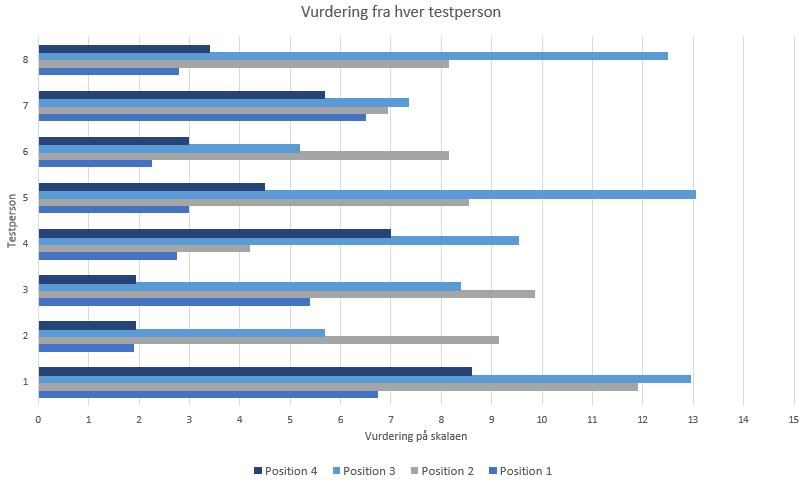
\includegraphics[width = \textwidth]{Figure/RaaDataTestpersoner.PNG} 
\caption{Rådata fra hver testperson. X-aksen er defineret ud fra den definerede skala-længde, hvorfor x-værdierne afspejler hvor indbydende testpersonen perciperer robotten. Testpersonerne er angivet på y-aksen.}
\label{fig:RaaDataTestpersoner}
\end{figure}
\noindent
%
\autoref{fig:RaaDataPositioner} er en sorting af data, som afspejler hvor indbydende hver testperson perciperer den specifikke hovedposition. 
%
\begin{figure}[H]
\centering
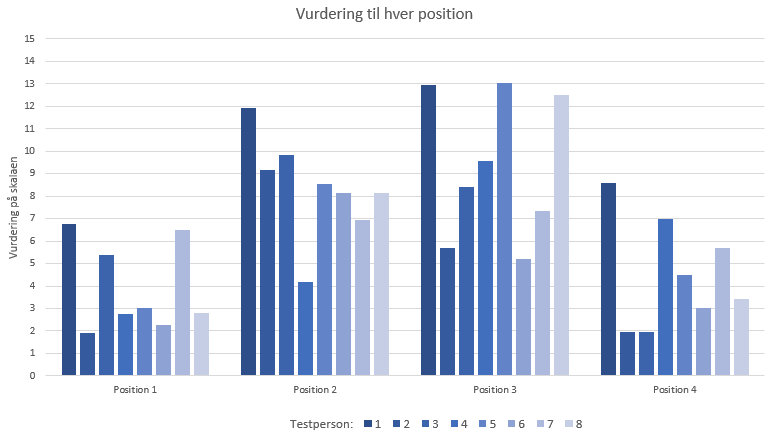
\includegraphics[width = \textwidth]{Figure/RaaDataPositioner.PNG} 
\caption{Rådata sorteret efter de fire hovedpositioner, repræsenteret på x-aksen, hvor y-aksen gengiver hvor indbydende hver testperson perciperer robotten afhængigt af hovedposition.}
\label{fig:RaaDataPositioner}
\end{figure}
\noindent
%
Med udgangspunkt i \autoref{fig:RaaDataPositioner} tyder det på, at både position 2 og position 3 perciperes som værende mere indbydende end både position 1 og position 4.\blankline
%
For at besvare hypoteserne, opstillet i \fullref{SkaleringseksperimentHypotese}, vil der i følgende afsnit udføres statistiske analyser.   


\section{Analyse}
\label{SkaleringseksperimentAnalyse}
%
Før analysen udføres, opstilles et boksplot for hver af de fire hovedpositioner, jævnfør \autoref{fig:boksplot}. Baseret på \autoref{fig:boksplot} tyder det på, at position 2 og position 3 begge perciperes som værende mere indbydende sammenlignet med position 1 og position 4.   
%
\begin{figure}[H]
\centering
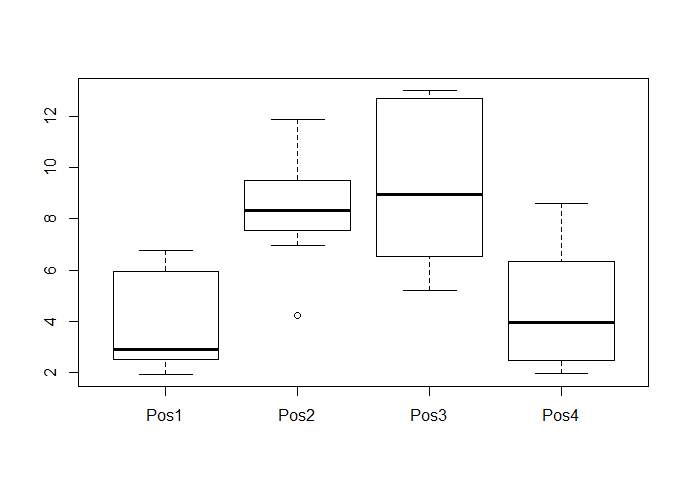
\includegraphics[width = 0.7\textwidth]{Figure/Rplot.png} 
\caption{Boksplot over hvor indbydende hver af de fire hovedpositioner perciperes.}
\label{fig:boksplot}
\end{figure}
\noindent
%
Data analyseres med en \textit{One-way Repeated Measures ANOVA}. Hvor \textit{one-way} refererer til antallet af uafhængige variable, som i dette tilfælde er én; robottens hovedposition. \textit{Repeated measures} refererer til, at samtlige testpersoner præsenteres for samtlige stimuli. Da formålet med denne test er at undersøge hvor indbydende en robot perciperes afhængigt af dens hovedposition, er den afhængige variabel testpersonernes individuelle respons angivet på skalaen. Den indsamlede data er af typen interval data, hvilket skyldes at VAS er en kontinuerlig skala. 

Ydermere dækker den uafhængige variabel over fire kategorier; de fire forskellige hovedpositioner, er det ligeledes oplagt at anvende en ANOVA, da det ønskes at sammenligne mere end to kategorier.\blankline
%
Følgende antagelser skal overholdes for at udføre en \textit{One-way Repeated Measures ANOVA}, \parencite[ss. 507-509]{PDF:ExploringAssumptions}: \blankline  
%
\begin{itemize}
	\item \textbf{Den afhængige variabel skal som minimum være målt på interval skala.}\\
	Vurderingen givet på skalaen er målt på en interval skala og opfylder dermed denne antagelse.
	\item \textbf{Der skal være homogen varians. }\\
	For at teste om der er homogen varians udføres \textit{Levene's test}. Testresultatet er $F(3.28)=1.09, p=0.37$, hvorfor der ikke er signifikant forskel og dermed er antagelsen om homogen varians opfyldt. 
	\item \textbf{Data skal være normalfordelt.}\\
	For teste om der er normalfordeling udføres en \textit{Shapiro-Wilk test}. Testresultatet er $W=0.94, p=0.09$, hvorfor der ikke er signifikant forskel og dermed er antagelsen om normalfordeling er opfyldt.
	\item \textbf{Uafhængig data.}\\
	Testpersonernes respons er uafhængige; testperson 1 har ikke indflydelse på de resterende testpersoners respons. Dog er der afhængighed mellem de fire konditioner testpersonerne præsenteres for.\blankline
\end{itemize}
\noindent
%
Da alle antagelser for at udføre en \textit{One-way Repeated Measures ANOVA} er opfyldt, udføres denne i \textit{rStudio}. Testresultatet er $F(3.21)=13,7, p=4.4*e^{-4}$, hvilket indikerer at der er signifikant effekt af robottens hovedposition på hvor indbydende robotten perciperes.

Baseret på dette resultat er det kun muligt at konkludere, at der er signifikant forskel mellem hvordan hovedpositionerne perciperes i forhold til hvor indbydende robotten er, det er derfor ikke muligt at afgøre hvor den signifikante forskel er. For at undersøge hvor forskellen er udføres der en \textit{Post Hoc test} af typen \textit{Pairwise Comparison}, hvilket udføres med t-tests, \parencite[s. 1171]{PDF:PairwiseComparison}. Testresultatet fremgår af \autoref{fig:sammenligning}.
%
\begin{figure}[H]
\centering
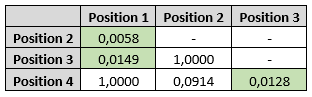
\includegraphics[width = 0.5\textwidth]{Figure/PostHocExcel.PNG} 
\caption{Sammenligning mellem vurderingerne af hvor indbydende robotten perciperes i henhold til dens hovedposition. Grøn markering angiver signifikante forskelle.}
\label{fig:sammenligning}
\end{figure}
\noindent
%
Baseret på \autoref{fig:sammenligning} fremgår det at både position 2 og position 3 er signifikant forskellige fra position 1. Sammenholdes dette med \autoref{fig:boksplot} kan det konkluderes at både position 2 og position 3 perciperes som værende mere indbydende end position 1. I tillæg er der signifikant forskel mellem position 3 og position 4, hvor position 3 perciperes som værende mere indbydende. Det er dog bemærkelsesværdigt at det ikke er tilfældet mellem position 2 og position 4, hvor der ikke fremgår en signifikant forskel, jævnfør \autoref{fig:sammenligning}.
%


\section*{Diskussion}
\label{Diskussion}
%
Foruden information omkring køn, alder og studieretning kunne det have været en fordel at måle testpersonernes højde, da den ene af testpersonerne, baseret på testledernes vurdering, var betydeligt højere end de resterende, samt en testperson, som var betydeligt lavere end de restende testpersoner. Disse højdeforskellen kan potentielt have en indflydelse på hvor indbydende testpersonerne perciperede robotten afhængigt af dens fire hovedpositioner. 

Under en samtale antages det, at samtalepartnerne generelt vil søge efter at opnå øjenkontakt og opretholde en form for øjenhøjde. Er dette tilfældet kan det ligeledes antages at robottens hovedposition positionelt har indflydelse på, hvorvidt testpersonerne betragter robotten som en form for samtalepartner og ydermere hvilke interaktionsmuligheder robotten tillader. Det vil derfor være interessant at undersøge sammenhængen mellem brugerens højde og hvor indbydende robotten perciperes afhængigt af hovedposition.\blankline  
%
Testpersonerne angav på en \textit{Visual Analogue Scale} (VAS), hvor indbydende de perciperede robotten afhængigt af dens hovedposition. Skalaen var designet med åbne endepunkter samt to ankerpunkter angivet med \textit{Slet ikke} og \textit{Ekstremt}. Som tidligere nævnt kommenterede testperson 1 i pilottesten at ankerpunktet \textit{Ekstremt} ikke var det mest passende ord at anvende som label, da det for testpersonen forbindes med at være attraktiv, hvilket testpersonen gav udtryk for robotter ikke er. Selvom det blev vurderet ikke at ændre på skalaen, kunne det have været en fordel at udføre gentagende pilottests for at undersøge om andre har en lignende holdning og på baggrund af det ændre labelen.    

Ydermere kan ordet \textit{ekstremt} også betragtes som værende et negativt ladet ord i den forstand, at det oftest benyttes til at beskrive kraftige vejrforhold, naturkatastofer eller politiske holdninger langt fra, hvad der antages for normalt, \parencite{WEB:Oxford}. Det kunne derfor have været en fordel at undersøge om der kunne findes en erstatning for \textit{Ekstremt} på den anvendte skala. Dog er en af fordelene ved at vælge et ord som \textit{Ekstremt}, at der formentlig ikke vil forekomme stimuli, der er endnu mere ekstreme end før. Taget i betragtning af at det andet ankerpunkt er \textit{Slet ikke}, hvor der det er svært at finde et alternativ som er mindre end slet ikke, så er det oplagt at vælge et ord til det andet ankerpunkt som dækker det samme. Med de to valgte ankerpunkter har det været muligt at dække hele skalaen, hvor hvis der var brugt \textit{Slet ikke} og \textit{Meget}, så ville der potentielt være stimuli som er mere end meget, hvorfor der formentlig vil forekomme samlinger omkring endepunktet, hvilket ikke har været tilfældet med de to valgte ankerpunkter.\blankline
%
Testpersonerne blev bedt om at vurdere hvor indbydende de perciperede robotten til hver af de fire hovedpositioner, hvor der antages en fælles forståelse for ordet \textit{indbydende}. Det blev observeret af testlederne, at et par af testpersonerne spurgte ind til hvad der mentes med indbydende, hvor testlederne var nødsaget til at uddybe forklaringen. En måde hvorpå der kunne skabes en form for fællesforståelse kunne have været, at præcisere yderligere hvor robotten er tiltænkt samt hvad dens formål er. Det kunne have indebåret en opgave, som testpersonerne skulle løse ved hjælp af robottens ansigt, som i det tilfælde skulle erstattes med en touchskærm. Ved at anvende en touchskærm kunne det potentielt have medvirket dels til en fælles forståelse for ordet \textit{indbydende} men også en forståelse for hvordan interaktionen med robotten foregår. \blankline
%
Testen blev kun udført af otte testpersoner, hvilket har indflydelse på præcisionen af de statiske analyser. Dette afspejles blandt andet af den store variation i respons, særligt ved position 2 og position 4, jævnfør \autoref{fig:boksplot}. Havde flere testpersoner deltaget kunne det have medført en mere pålidelig sammenhæng mellem hvor indbydende robotten perciperes afhængigt af dens hovedposition. 




\section{Konklusion}
\label{SkaleringseksperimentKonklusion}
%
Position 2 (65$^{\circ}$) og position 3 (35$^{\circ}$) blev begge vurderet til at være mere indbydende end position 1 og position 4, som generelt blev vurderet på skalaens nedrehalvdel. Der blev udført en \textit{One-way Repeated Measures ANOVA}, som indikerede at der forekommer en signifikant forskel mellem hovedpositionerne i forhold til hvor indbydende robotten perciperes. Efterfølgende blev der foretaget en \textit{Pairwise Comparison}, hvorfra det blev fundet, at der er signifikant forskel mellem position 1 og position 2, mellem position 1 og position 3, samt en forskel mellem position 3 og position 4. Baseret på resultaterne er det muligt at afvise nul hypotesen, $H_0$, jævnfør \fullref{SkaleringseksperimentHypotese}. Der er dog ikke endegyldigt belæg for at acceptere den alternative hypotese, $H_a$, da der ikke er fundet en signifikant forskel mellem position 2 og position 4. 

Dog kan det konkluderes, at for at robotten perciperes mest indbydende, i forhold til de fire valgte hovedpositioner, skal den være indstillet enten i position 2 eller i position 3. Dette gengiver at robottens hovede er vinklet skråt opad, hvilket formentlig giver testpersonerne i følelse af, at de har øjenkontakt med den.       







\newcommand{\UdviklingAfSkalapartname}{Udvikling af skala123}
\newcommand{\UdviklingAfSkalaparttext}{

Det er her vi finder ud af hvad folk rent faktisk siger omkring den her robot, hvor vi er i lufthavnen og laver en eller anden form for observations studie af dem og analyserer data med affinity diagrammer og generelt hele processen omkring at udvikle vores skalaer.
\newpage 
}
%
\part[\UdviklingAfSkalapartname]{\UdviklingAfSkalapartname
\label{\UdviklingAfSkalapartname}
\vspace{8mm}
	\begin{center}
		\begin{minipage}[l]{14cm}
			\textnormal{\normalsize\noindent\UdviklingAfSkalaparttext}
		\end{minipage}
	\end{center}
}
	\chapter{Parametre med indflydelse på sociale robotter}
\label{ParametreSocialeRobotter}
%
Formålet med denne undersøgelse er, at få folk til at sætte deres egne ord på oplevelsen af interaktionen med en social robot. Herefter er ønsket at bruge testpersonernes egne ord til at forstå hvilke parametre, der er vigtige at tage højde for, når sociale robotter skal designes. Her er det ikke nødvendigvis vigtigt at undersøge, om en given interaktion fungerer, men nærmere hvordan den skal være for at fungere. For at finde ud af, hvordan reelle brugere snakker om robotten i den rigtige kontekst, opstilles et feltstudie i en lufthavn. Det vælges at benytte Aalborg Lufthavn til dette feltstudie, da kontakt og aftaler med Københavns Lufthavn er tidskrævende og ikke nødvendigvis kan ske inden for projektets tidsperiode. Ydermere er det nemmere at transportere robotten til Aalborg Lufthavn og der er mere ro i lufthavnen til at køre faktiske tests.\blankline
%
Feltstudier, hvor brugerne mødes ude i den virkelig verden, kan ofte give et bedre billede af hvordan brugere faktisk interagerer med produkter. Det kan også afsløre nogle af de problemer eller holdninger til produktet, som ikke bliver opdaget i mere kliniske tests. I denne test vælges det at testpersonerne skal interagere med robotten, hvorefter de vil blive bedt om at fortælle om deres oplevelse, hvilket vil blive uddybet yderligere i de følende afsnit.

\section{Metode}
\label{ParametreMetode}
%
Følgende afsnit beskriver, hvordan robotten præsenteres for testpersonerne, hvordan interaktionen skal foregå samt hvilke metoder, der bruges for at få den relevante information fra testpersonerne.\blankline
%
Noget om kvalitativ metode/eksploration og feltstudier/kontekst?\blankline 
%Projektet kigger på interaktionen og det sociale aspekt i robotter tilknyttet en lufthavn, hvorfor det er relevant at opstille et scenarie baseret på en lufthavns situation og med brugere, der benytter lufthavnen.

Da inspirationen til den sociale robot kommer mere eller mindre fra Double, vælges det at bruge denne til testen. Udover at inspirationen kommer herfra, så kan det påvirke folk betydeligt om de interagerer med en færdig robot eller en prototype, der hverken har det rigtig udseende eller de rigtige bevægelser. For at testpersonerne kan forstå, hvordan robotten skal opføre sig, specielt med en mere dynamisk bevægelse, vælges det at bruge Double i stedet for at sætte prototypen på en robotstøvsuger og fjernstyre denne. 

\subsection{Fremgangsmåde}
\label{ParametreFremgangsmaade}
%
For at teste hvilke parametre, der er vigtige i en social robot skal robotten præsenteres for testpersonerne, hvorefter de skal medvirke i et interview, for at få sat ord på deres oplevelse med robotten. 

Da det ønskes at observere testpersonernes umiddelbare reaktion på deres første møde med robotten, bruges den også til at rekruttere testpersoner med. Det foregår ved, at robotten kører hen til mennesker i Aalborg Lufthavn og via skærmen spørger folk, om de har lyst til at deltage i en test. Det vælges derudover at robotten skal køre hen til folk på denne måde, for at give testpersonerne en reel oplevelse af, at robotten kommer hen og henvender sig til dem på et tidspunkt, hvor de ikke er opmærksomme på at de er en del af en undersøgelse. Dem der indvilligere i at deltage i testen følger efter robotten over til vores testområde, hvor testpersonerne mødes med testlederen for første gang.\blankline

Det er vigtigt at der skabes en afslappet stemning, hvor testpersonerne føler sig trykke ved at udtrykke sig og fortælle om oplevelsen med robotten, samtidig med at de ikke føler de spilder dyrebar tid eller bliver stressede over at skulle nå et fly. For at skabe en god stemning, tilbydes testpersonerne en kop kaffe og det er muligt at small-talke omkring eksepelvis hvor testpersonerne skal rejse hen eller har været henne. Selvom det kan virke unødvendigt, er det vigtigt at der bruges lidt tid på denne del af testen, for at sikre at testpersonen føler sig i trygge rammer. 

Når en god stemning er skabt fortæller testlederen om formålet og fremgangsmåden med testen, og testen bedes læse og underskrive en samtykkeerklæring, vedlagt i \fullref{APP:Samtykkeerklaering}.\blankline
%

Selve interaktionen med robotten foregår med en \textit{"Wizard of Oz"} tilgang, hvor en person styrer robotten fra sin computer. Robotføreren sidder ved et bord i nærheden, så vidt muligt bag ved testpersonen, for ikke at tiltrække opmærksomhed. Hvis testpersonen spørger ind til robotføreren får de forklaret, at vedkommende er der for at notere observationer undervejs. 
\textbf{FIND UD AF HVILKEN INTERAKTION BRUGEREN SKAL HAVE MED ROBOTTEN, BASERET PÅ HVILKE BRUGSSCENARIER DER KAN VÆRE I LUFTHAVNEN} \blankline
%
Efter testpersonen er blevet præsenteret for og har interageret med robotten og den kontekst hvori robotten skal fungere, findes det relevant at interviewe testpersonen, for på den måde at forstå hvordan de tænker omkring sociale robotter. Der stilles brede og åbne spørgsmål, for at få testpersonen til at starte med at tale frit. Interviewet med testpersonen optages \textbf{(Eller filmes?)}, for til databehandlingen at kunne nedskrive udtalelser, opbygge et affinitydiagram og på den måde udlede hvilke parametre ved en social robot, der er vigtige for testpersonerne.

\section{Samtaleemner}
\label{ParametreSamtaleemner}
%
Det er her vi skal skrive hvilke spørgsmål vi tænker at stille de rejsende og måske hvorfor vi strukturer vores interview på den måde og hvorfor de spørgsmål er relevante. 


\section{Testpersoner}
\label{TestAfSkalaTestpersoner}
%

\section{Relaterede studiers test af parametre}
\label{ParametreTidligereStudier}
% Jeg ved ikke om denne sektion skal være der..
Mange undersøgelser laves bare med spørgeskemaer, likert-skalaer, korte interaktioner med robotten, videoklip med robotten. 

Inddrag Personality of social robots perceived through the appearances.

Kom ind på hvordan det måles, hvad har andre gjort i forhold til det (overvej om det skal være en sektion for sig selv).\blankline


Out of the five widely used personality dimensions, namely the extroversion, agreeableness, conscientiousness, neuroticism, and openness [5], the most important dimensions for social interactions are those that concern individual differences in social behavior, namely extroversion and agreeableness or their common rotations, ‘friendliness’ and ‘dominance’ [6]. Fra Personality of social robots perceived trough the appearance side. 272.


\newcommand{\RobotBevaegelsepartname}{Robot bevaegelse/Henvendelse}
\newcommand{\RobotBevaegelseparttext}{Her skal vi finde ud af præcis hvordan robotten skal bevægelse (altså bevægelses mønstret), hvor hurtigt den skal bevæge sig, hvornår den skal stoppe samt hvilken retning den skal komme fra. 
\newpage 
}
%
\part[\RobotBevaegelsepartname]{\RobotBevaegelsepartname
\label{\RobotBevaegelsepartname}
\vspace{8mm}
	\begin{center}
		\begin{minipage}[l]{14cm}
			\textnormal{\normalsize\noindent\RobotBevaegelseparttext}
		\end{minipage}
	\end{center}
}
\chapter{Robot bevægelse}
\label{RobotBevaegelse}
%
Skriv lidt om hvordan robotten "bør" bevæge sig - brug kilder fra interaktion med sociale robotter og sæt tests op hvor vi tester stop afstand og hastighed. \blankline
%
\section{Test idé}
%
Vi tager udgangspunkt i kilderne: Close But Not Stuck:
Understanding Social Distance in Human-Robot Interaction Through a Computer Mediation Approach, SKRIV FLERE KILDER. De bruger en robot der bevæger sig mellem 0,9 km/h og 1,44 km/h og har en stop afstand på 50cm $\pm$ 10 cm, den undersøgelse blev lavet i England og fokuserer på tre retninger robotten kan kommer fra: Venstre, højre og frontalt, det er alt sammen i forhold til når testpersonen sidder ned. Stop afstanden afhænger SUPER meget af kultur de 50 cm kommer fra hvor tæt folk i England (måske generelt for flere europæiske lande - nok ikke syd europa) kommer på hinanden ved menneske-menneske interaktion, hvorimod i de fleste asiatiske kulturer er den afstand altså kun mellem 20-30 cm. Da vi jo har en lufthavn hvor nærmest alle nationaliteter kan være præsenteret er det vigtigt at vi tænker over det. I forhold til hastigheden mener testpersonerne at det er "about right" eller for langsomt, hvorfor jeg forestiller mig at vi kan bruge deres hastigheder som start og så øge hastigheden og få testpersonerne til at vurdere hvordan det er. Det kan gøres på flere måder - skala, mundtligrespons osv. 

Vi skal selvfølgelig give dem konteksten og jeg tænker det skal være så simpelt som muligt da dette kun er en indledende test. Det jeg forestiller mig er at vi kunne fokuserer på når robotten henvender sig til en person, i og med robotten på forhånd jo ikke nødvendigvis ved hvad den skal hjælpe personen med. 




\newcommand{\TestAfSkalapartname}{   Udvikling af skala til evaluering af HRI}
\newcommand{\TestAfSkalaparttext}{For at besvare den anden problemstilling: \textit{Hvordan kan de fundne parametre gengives i skalaer, som efterfølgende kan bruges til at evaluere HRI?}, vil det først forsøges at udvikle de nødvendige skalaer, der bygger på spørgsmål, som vedrører de specifikke parametre. Dernæst vil der udføres endnu en undersøgelse i Aalborg Lufthavn, hvor de rejsende skal evaluere HRI ved hjælp af de udviklede skalaer. 
\newpage 
}
%
\part[\TestAfSkalapartname]{\TestAfSkalapartname
\label{\TestAfSkalapartname}
\vspace{8mm}
	\begin{center}
		\begin{minipage}[l]{14cm}
			\textnormal{\normalsize\noindent\TestAfSkalaparttext}
		\end{minipage}
	\end{center}
}


%%%% Kilder %%%%
\printbibliography	%Litteraturlisten inkluderes

%%%% Bilag %%%%
%\appendix
%\appendixpage

%%Skriv dokumentet ind

%\chapter{Raw data}
\label{app:Data}

%\begin{figure}[H]
%	\centering
%	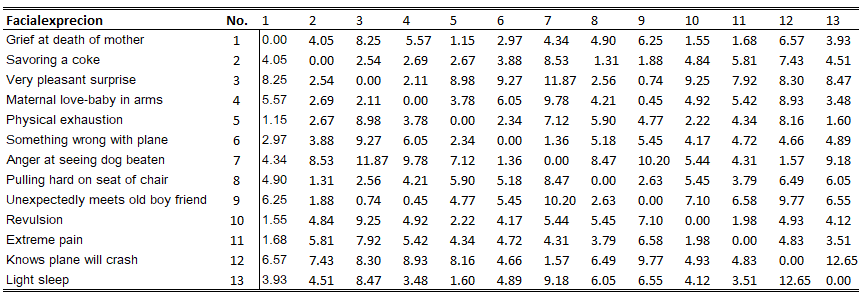
\includegraphics[resolution=300,width=0.8\textwidth]{Figure/Data}
%	\caption{Raw data from the test}
%	\label{fig:Data}
%\end{figure}
%\noindent





\end{document}
 